\chapter{Background}
\label{chap:background}

This chapter introduces the concepts needed to understand the proposed methodology: the physical and numerical framework of Rayleigh--Taylor instability, dimensionality reduction through Fourier and wavelet representations, and the principles of score-based diffusion models.

\section{Physical and Numerical Framework}

\section{Rayleigh--Taylor Instability}

\subsection{Physical Mechanism}

The Rayleigh--Taylor instability (RTI) is a hydrodynamic instability that occurs when a dense fluid is accelerated by a lighter one. Under such conditions, perturbations located at the interface between the two fluids may grow over time and generate complex non-linear flow structures.

This instability appears in many physical systems involving strong density gradients and acceleration effects, including astrophysical flows, supernova explosions, atmospheric phenomena, and inertial confinement fusion plasmas. In the context of high-energy-density physics, RTI plays a major role because it can strongly enhance turbulent mixing and degrade the stability of compressible flows.

In inertial confinement fusion configurations, the instability develops during the implosion phase when the dense shell material is accelerated inward by the pressure generated by the ablation of the outer surface. Small imperfections initially present on the capsule surface are amplified during compression and progressively distort the interface.

\begin{figure}[H]
\centering
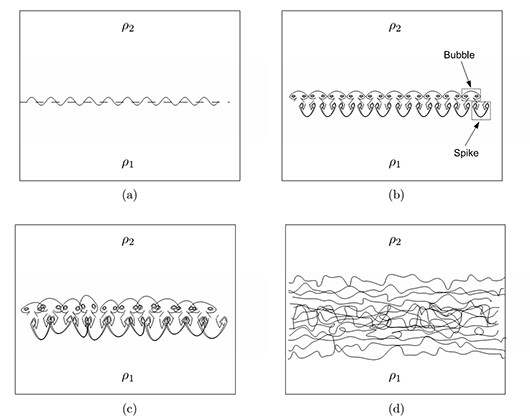
\includegraphics[width=0.55\textwidth]{figures/ch1/rti_sketch.png}
\caption{Illustration of evolution of the Rayleigh--Taylor instability at the interface between two fluids of different densities}
\label{fig:rti_principle}
\end{figure}

As the instability evolves, the interface develops characteristic structures commonly referred to as \textit{bubbles} and \textit{spikes}. The lighter fluid penetrates the denser region through rising bubbles, while the denser fluid penetrates downward through spikes. At later stages, non-linear interactions between structures lead to the formation of increasingly complex flow patterns and eventually to turbulent mixing.

The growth of RTI strongly depends on several physical parameters, including the density contrast between the two fluids, the acceleration field, the viscosity, compressibility effects, and the initial perturbation spectrum. One important dimensionless quantity used to characterize the instability is the Atwood number~\citep[p.~22]{zhou2017rti1}, defined as

\begin{equation}
    A = \frac{\rho_h - \rho_l}{\rho_h + \rho_l}
\end{equation}

where $\rho_h$ and $\rho_l$ denote the densities of the heavy and light fluids respectively. Large Atwood numbers generally correspond to stronger instability growth.


\subsection{Mathematical Origin of the Rayleigh--Taylor Instability}

The Rayleigh--Taylor instability naturally arises from the governing equations of fluid motion when a density stratification is subjected to an acceleration directed from the heavier fluid toward the lighter one. Following the classical development of Kull~\cite{KULL1991197}, the instability can be understood by considering the evolution of small perturbations of an initially hydrostatic equilibrium.

For an incompressible Newtonian fluid, the conservation equations read

\begin{align}
\nabla\cdot\mathbf{u} &= 0,\\
\rho\left(
\frac{\partial\mathbf{u}}{\partial t}
+\mathbf{u}\cdot\nabla\mathbf{u}
\right)
&=
-\nabla p
+\mu\nabla^2\mathbf{u}
+\rho\mathbf{g},
\end{align}

where $\rho$ denotes the density, $\mathbf{u}$ the velocity field, $p$ the pressure and $\mathbf{g}$ the imposed acceleration.

In the absence of motion, the system is in hydrostatic equilibrium,

\begin{equation}
\nabla p_0=\rho\mathbf{g}.
\end{equation}

The stability of this equilibrium depends entirely on the density stratification. When the lighter fluid lies above the heavier one, any perturbation is counteracted by the buoyancy force and the equilibrium is stable. Conversely, when the heavier fluid overlies the lighter one, a small displacement of the interface produces a buoyancy force that amplifies the perturbation rather than restoring it. The hydrostatic equilibrium therefore becomes unstable.

Following the linear stability analysis presented by Kull~\cite{KULL1991197}, the flow variables are decomposed into a base state and infinitesimal perturbations,

\begin{equation}
\mathbf{u}=\mathbf{u}',
\qquad
p=p_0+p',
\qquad
\rho=\rho_0+\rho',
\end{equation}

where only first-order terms are retained. Assuming perturbations of normal-mode form,

\begin{equation}
\exp\left(i\mathbf{k}\cdot\mathbf{x}+\gamma t\right),
\end{equation}

the linearized equations reduce to an eigenvalue problem whose solution provides the perturbation growth rate.

For the ideal case of two incompressible, inviscid fluids separated by a sharp interface and neglecting surface tension, the classical dispersion relation is

\begin{equation}
\gamma^2=Agk,
\end{equation}

The positive sign of $\gamma^2$ demonstrates that disturbances grow exponentially with time,

\begin{equation}
\eta(t)=\eta_0e^{\gamma t},
\end{equation}

revealing that the hydrostatic equilibrium is intrinsically unstable when the acceleration is directed from the heavy fluid toward the light one. This result constitutes the mathematical foundation of the Rayleigh--Taylor instability and explains why small perturbations evolve into the nonlinear structures observed experimentally and numerically.




\subsection{Linear and Non-linear Regimes}

During the early stages of the instability, perturbations remain sufficiently small for linear stability theory to apply. In the incompressible inviscid limit, the perturbation amplitude grows exponentially with growth rate~\citep[p.~23]{zhou2017rti1}

\[
\gamma = \sqrt{A g k},
\]

where $A$ is the Atwood number, $g$ the acceleration, and $k$ the perturbation wavenumber.

As the perturbation amplitude increases, non-linear effects progressively become dominant. Mode coupling mechanisms appear and coherent structures interact across multiple spatial scales. The flow then transitions toward a turbulent mixing regime characterized by strong intermittency and multi-scale dynamics.

% \begin{figure}[htbp]
% \centering
% \fbox{
% \parbox[c][6cm][c]{0.85\textwidth}{
% \centering
% Placeholder for RTI temporal evolution figure
% }}
% \caption{Typical evolution of the Rayleigh--Taylor instability from the linear regime toward turbulent mixing.}
% \label{fig:rti_evolution}
% \end{figure}

This transition from ordered interface perturbations to fully developed turbulent structures constitutes one of the main scientific challenges associated with RTI simulations. The large range of dynamically relevant scales makes accurate numerical prediction particularly difficult.

\subsection{Multi-scale Nature and Turbulence}

One of the main characteristics of the Rayleigh--Taylor instability is its strongly multi-scale behavior. Large coherent structures generated during the non-linear growth phase progressively fragment into smaller vortical structures through turbulent cascades and interface stretching mechanisms.

As turbulence develops, energy is transferred across a wide range of spatial scales. Fine-scale structures emerge near the mixing layer interface and interact continuously with larger coherent motions. This scale coupling significantly complicates both physical analysis and numerical modeling.

\begin{figure}[H]
\centering
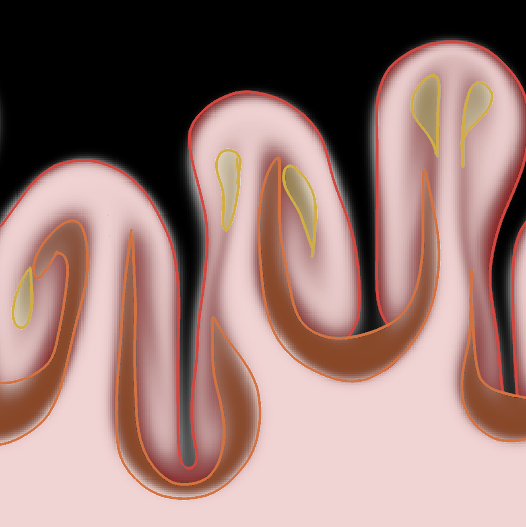
\includegraphics[width=0.30\textwidth]{figures/ch1/RT-MultiScale.png}
\caption{Example of multi-scale structures generated during the turbulent phase of the Rayleigh--Taylor instability}
\label{fig:rti_multiscale}
\end{figure}

The presence of coherent structures, intermittent mixing regions, and localized gradients motivates the use of multi-resolution analysis tools capable of simultaneously capturing both spatial localization and scale-dependent information. This aspect will later motivate the investigation of wavelet-based representations for generative modeling purposes.

\section{Dimensionality Reduction and Multi-scale Representations}

\section{Motivation}

The density fields generated by Direct Numerical Simulations of the Rayleigh--Taylor instability contain a large amount of spatial information distributed across multiple scales. As discussed in the previous chapter, the instability evolves from relatively smooth interface perturbations toward highly complex turbulent structures characterized by sharp gradients, coherent vortices, and intermittent mixing regions.

From a machine learning perspective, directly learning probability distributions in such high dimensional spaces is particularly challenging. The dimensionality of the data increases rapidly with the spatial resolution of the simulations, leading to high memory requirements and expensive training procedures. Moreover, the limited number of DNS samples available further complicates the learning process, since the model may tend to memorize the training examples rather than learn patterns that generalize to unseen samples.

Reducing the dimensional complexity of the data while preserving the physically relevant structures therefore constitutes an important objective. Beyond computational considerations, appropriate representations may also improve the stability and efficiency of generative models by emphasizing dominant structures and reducing redundant information.

Another important aspect concerns the strongly multi-scale nature of RTI flows. Large coherent structures coexist with fine turbulent features and localized interface deformations. Consequently, representations capable of simultaneously capturing both large-scale organization and localized high-frequency structures are particularly attractive.

Several approaches can be considered for this purpose. Classical spectral decompositions based on Fourier transforms provide efficient global frequency representations and are widely used in turbulence analysis. However, they remain limited when dealing with localized or strongly discontinuous structures. Multi-resolution methods based on wavelet transforms constitute an alternative approach capable of jointly representing spatial localization and scale-dependent information.

The objective of this chapter is therefore to introduce the different representations investigated in this work and to analyze their respective advantages and limitations in the context of Rayleigh--Taylor instability fields.

\section{Fourier Transform}

\subsection{Spectral Decomposition}

Fourier transforms constitute one of the most widely used tools for the analysis of turbulent flows and physical fields. The main idea consists in representing a signal as a superposition of sinusoidal modes associated with different spatial frequencies.

For a one- or two-dimensional scalar field $f(x,y)$, where $x$ and $y$ are the spatial coordinates, the Fourier transform is defined as


\begin{align}
    1D&: \hat{f}(k_x) = \int f(x) e^{-i k_x x} dx, \\
    2D&: \hat{f}(k_x,k_y) = \int\int f(x,y) e^{-i(k_x x + k_y y)} dx dy,  
\end{align}
where $(k_x,k_y)$ denote the spatial frequency components.

The Fourier transform can be interpreted as a projection of a signal onto a basis of globally supported sinusoidal functions. Therefore, the original field can be expressed as a linear combination of Fourier modes weighted by the corresponding spectral coefficients $\hat{f}(k_x,k_y)$. It is also possible to perform a non-linear reconstruction by retaining only the largest coefficients, as illustrated in Figure \ref{fig:fourier_decomposition}. The linear and non-linear reconstructions can be expressed as follows:

\begin{align}
    \text{Basis} &: F = \left\{ \phi_k \mid k\in\mathbb{Z},\ \phi_k(x) = e^{2\pi i k x} \right\}, \\
    \text{Linear} &: f_K(x)=\sum_{ |k| \le K }\langle f, \phi_k \rangle \phi_k(x), \\
    \text{Non-linear} &: f_H(x)=\sum_{ k \in \Lambda_H } \langle f,\phi_k \rangle \phi_k(x),
    \quad \Lambda_H=\left\{ k \mid |\langle f, \phi_k \rangle| \ge H \right\}.
\end{align}


\begin{figure}[ht]
    \centering

    \begin{minipage}{0.8\textwidth}
        \centering
        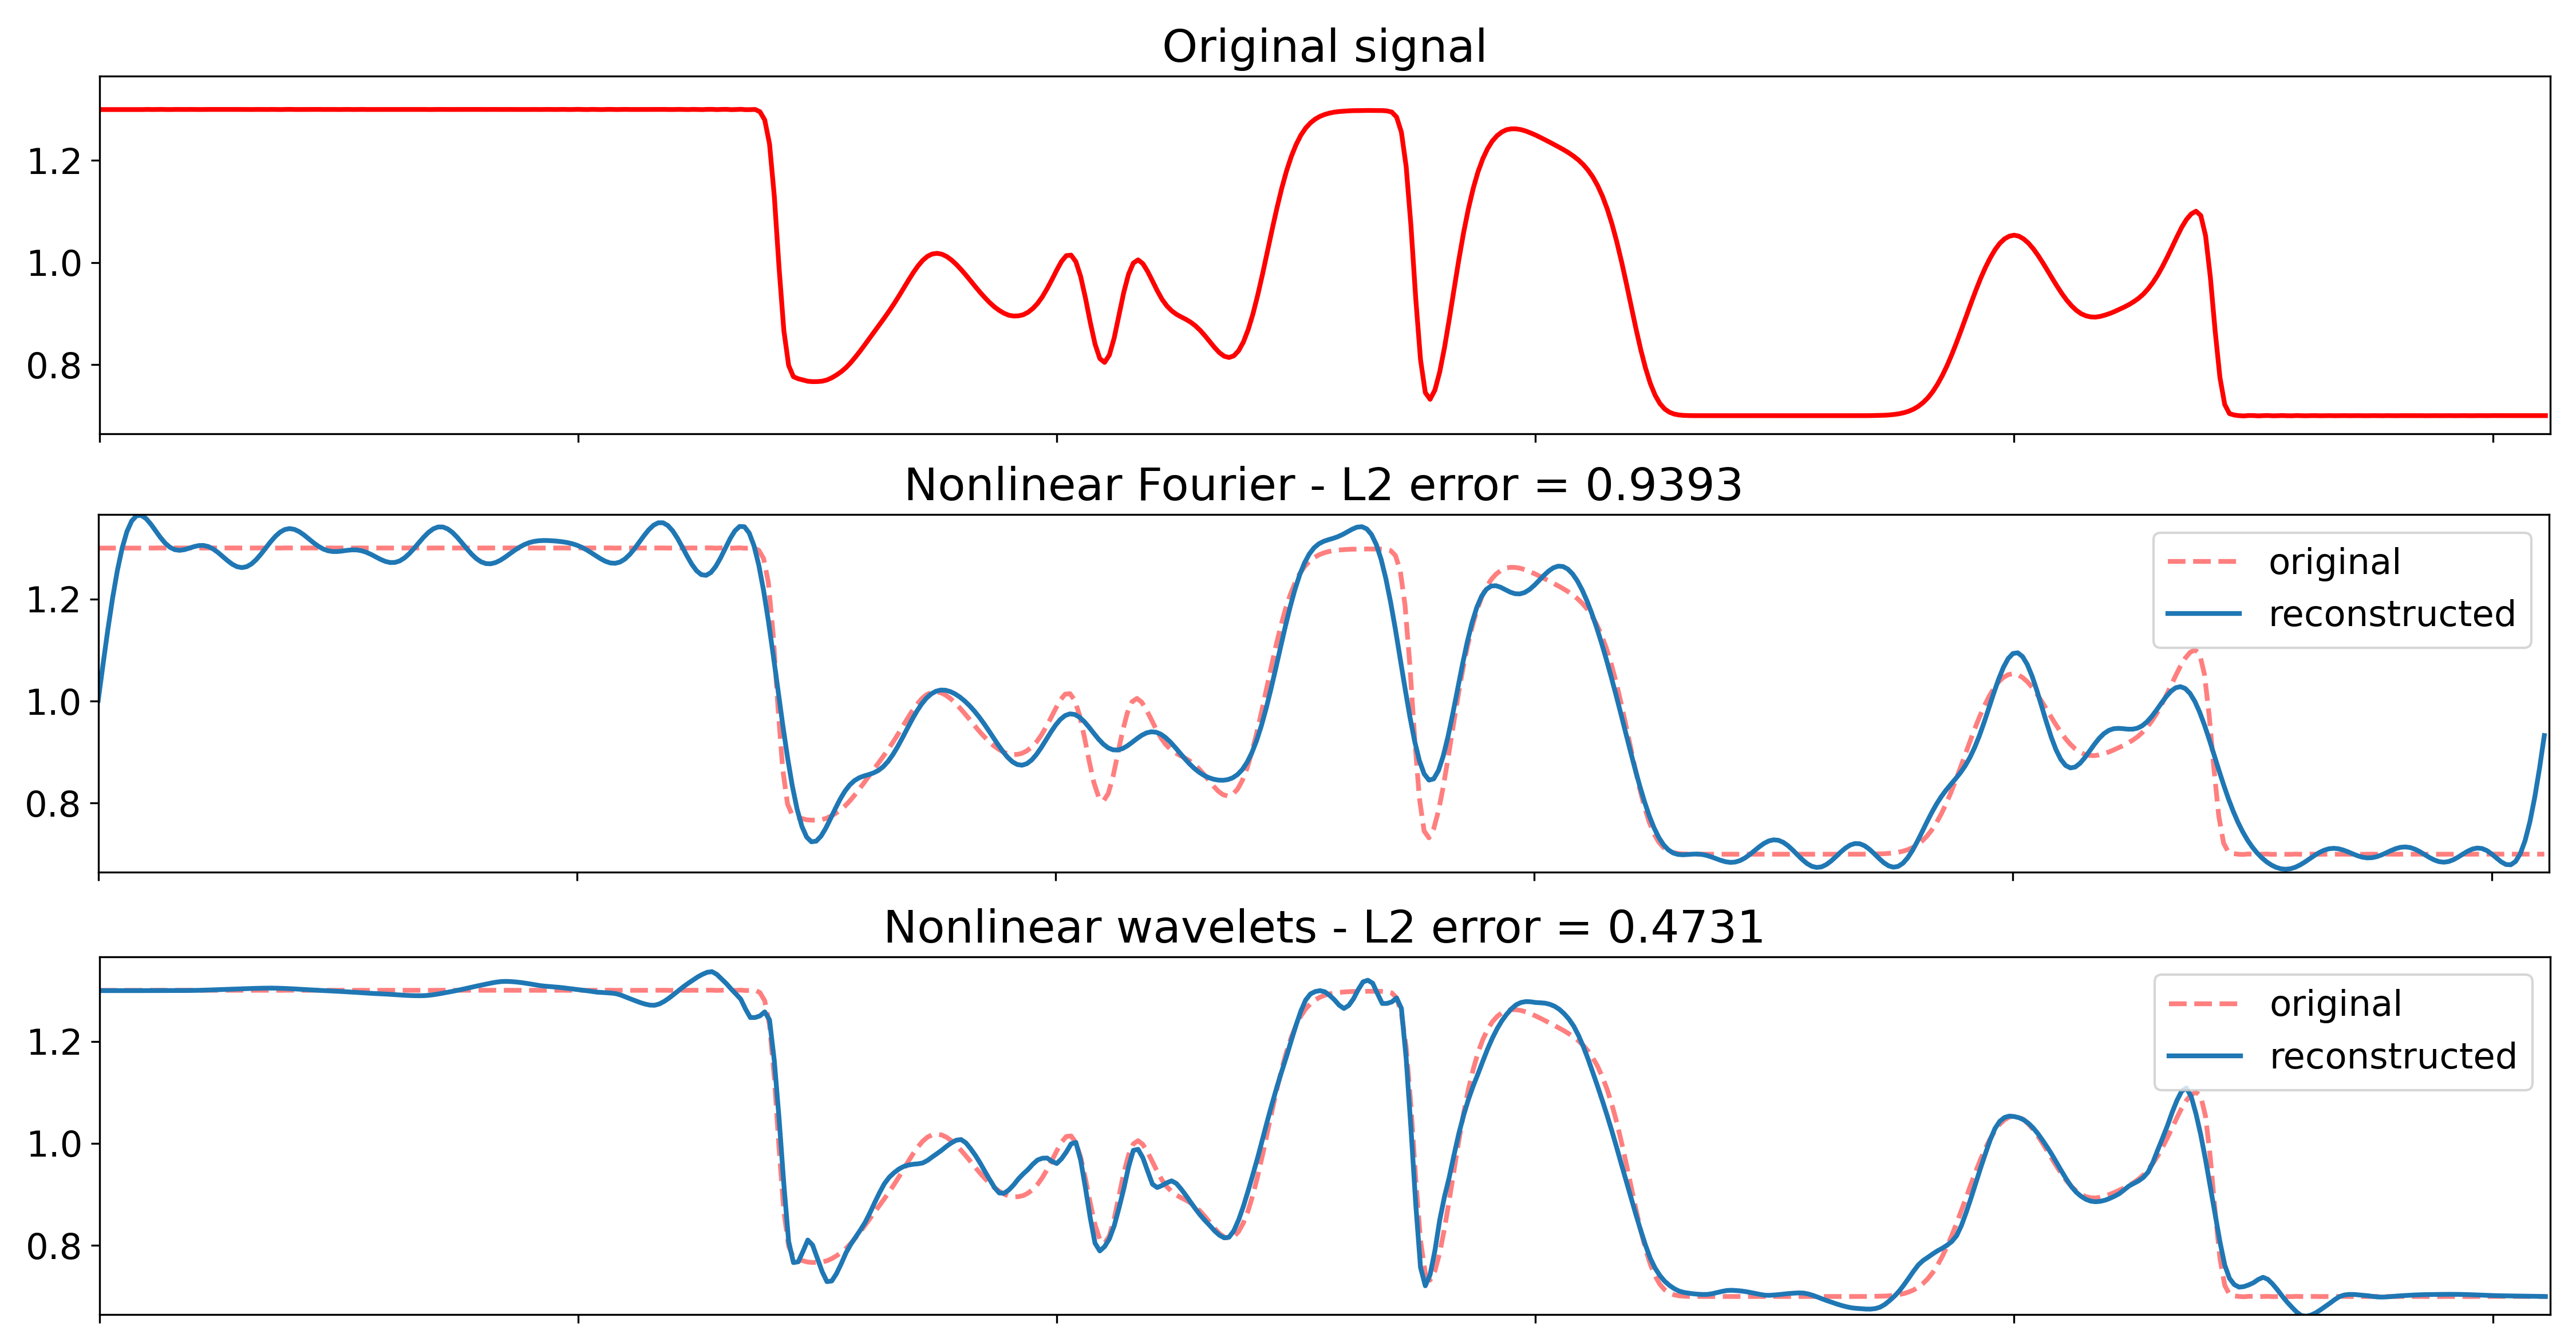
\includegraphics[width=\linewidth]{figures/ch2/sig.png}

        \vspace{0.3em}

        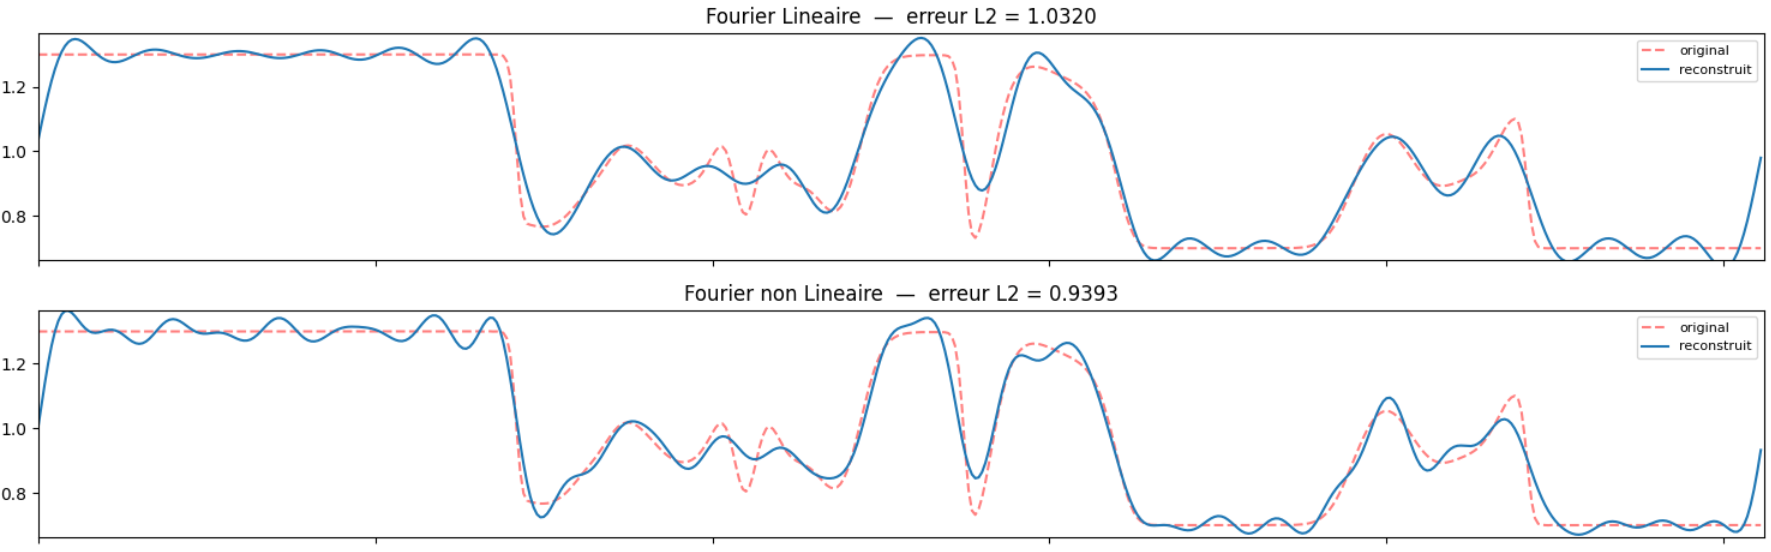
\includegraphics[width=\linewidth]{figures/ch2/fourier.png}
    \end{minipage}

    \caption{Illustration of a Fourier decomposition with 45 modes of a one-dimensional density field.}
    \label{fig:fourier_decomposition}
\end{figure}


In turbulence studies, Fourier analysis is particularly useful because it naturally describes the distribution of energy across spatial scales. Low-frequency modes correspond to large coherent structures, while high-frequency modes represent fine turbulent fluctuations.

\subsection{Advantages for Turbulence Analysis}

Spectral methods possess several important advantages for the analysis of fluid flows. First, Fourier transforms provide compact representations for smooth periodic signals. Second, many physical quantities of interest, such as energy spectra, can be directly expressed in spectral space.

In the context of DNS, pseudo-spectral solvers themselves are often formulated using Fourier representations because of their high numerical accuracy and low dissipation properties. Consequently, Fourier analysis naturally appears as a first candidate for dimensionality reduction and feature extraction.

Furthermore, spectral filtering techniques make it possible to separate structures according to their characteristic scales, which is particularly relevant for turbulent flows exhibiting cascade mechanisms.

\subsection{Limitations for Localized Structures}

Despite their numerous advantages, Fourier representations also exhibit important limitations when dealing with localized or non-smooth structures. Since Fourier basis functions extend over the entire spatial domain, local modifications of the signal affect all spectral coefficients simultaneously. As a consequence, sharp gradients and localized discontinuities generally require a large number of Fourier modes to be accurately reconstructed.

This limitation is closely related to the Gibbs phenomenon, which appears when truncated Fourier series are used to approximate signals containing discontinuities or strong localized variations. Near sharp interfaces, oscillatory artifacts emerge and persist even when increasing the number of retained modes.

\begin{figure}[htbp]
\centering
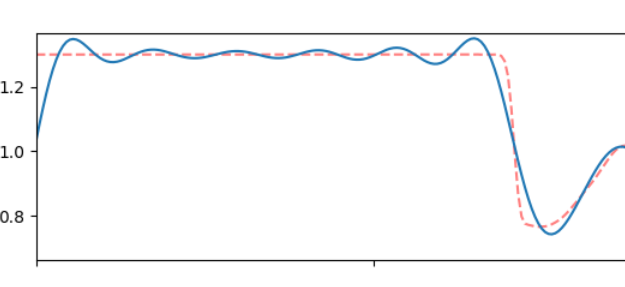
\includegraphics[width=0.65\textwidth]{figures/ch2/gibbs.png}
\caption{Illustration of the Gibbs phenomenon near a discontinuity reconstructed using a truncated Fourier representation.}
\label{fig:gibbs}
\end{figure}

Although RTI density fields are not strictly discontinuous, they contain steep density gradients, localized interface deformations, and intermittent turbulent structures that exhibit similar reconstruction difficulties. Capturing such localized features using Fourier modes may therefore require a large number of coefficients, reducing compression efficiency and increasing the complexity of the representation.

In addition, Fourier decompositions provide limited spatial localization information. While they accurately describe the global frequency content of the flow, they do not directly indicate where specific structures are located in physical space. This limitation becomes particularly important for turbulent RTI fields, where coherent structures and mixing regions evolve dynamically and remain strongly localized.

These observations motivate the investigation of multi-resolution approaches capable of simultaneously representing both scale-dependent information and spatial localization properties.


\section{Wavelet Transform}

\subsection{Continuous Wavelet Transform}
Wavelet transforms provide a representation framework capable of simultaneously capturing spatial localization and scale-dependent information. The mathematical foundation of wavelet analysis is the \textit{Multi-resolution Analysis} (MRA), introduced by Mallat~\citep[p.~22]{Mallat2009} and Meyer~\citep[p.~22]{Meyer1992}. An MRA is constructed from a scaling function $\phi$, also called the father wavelet, which spans a hierarchy of nested approximation spaces.

Unlike Fourier transforms, which use globally supported sinusoidal basis functions, wavelet transforms employ functions with compact support that can be created by dilation and translation of a mother wavelet $\psi$. We can then define a wavelet as a function of zero mean:
\begin{align}
    \int_{-\infty}^{\infty} \psi(x) dx = 0
\end{align}
The wavelet family is then defined as:
\begin{align}
    \psi_{u,s}(x) = \frac{1}{\sqrt{s}} \psi\left(\frac{x-u}{s}\right)
\end{align}
where $u \in \mathbb{R}$ is the translation parameter and $s > 0$ is the scale parameter. A few examples of wavelet generating functions are shown in Figure \ref{fig:wavelets}.

\begin{figure}[H]
\centering
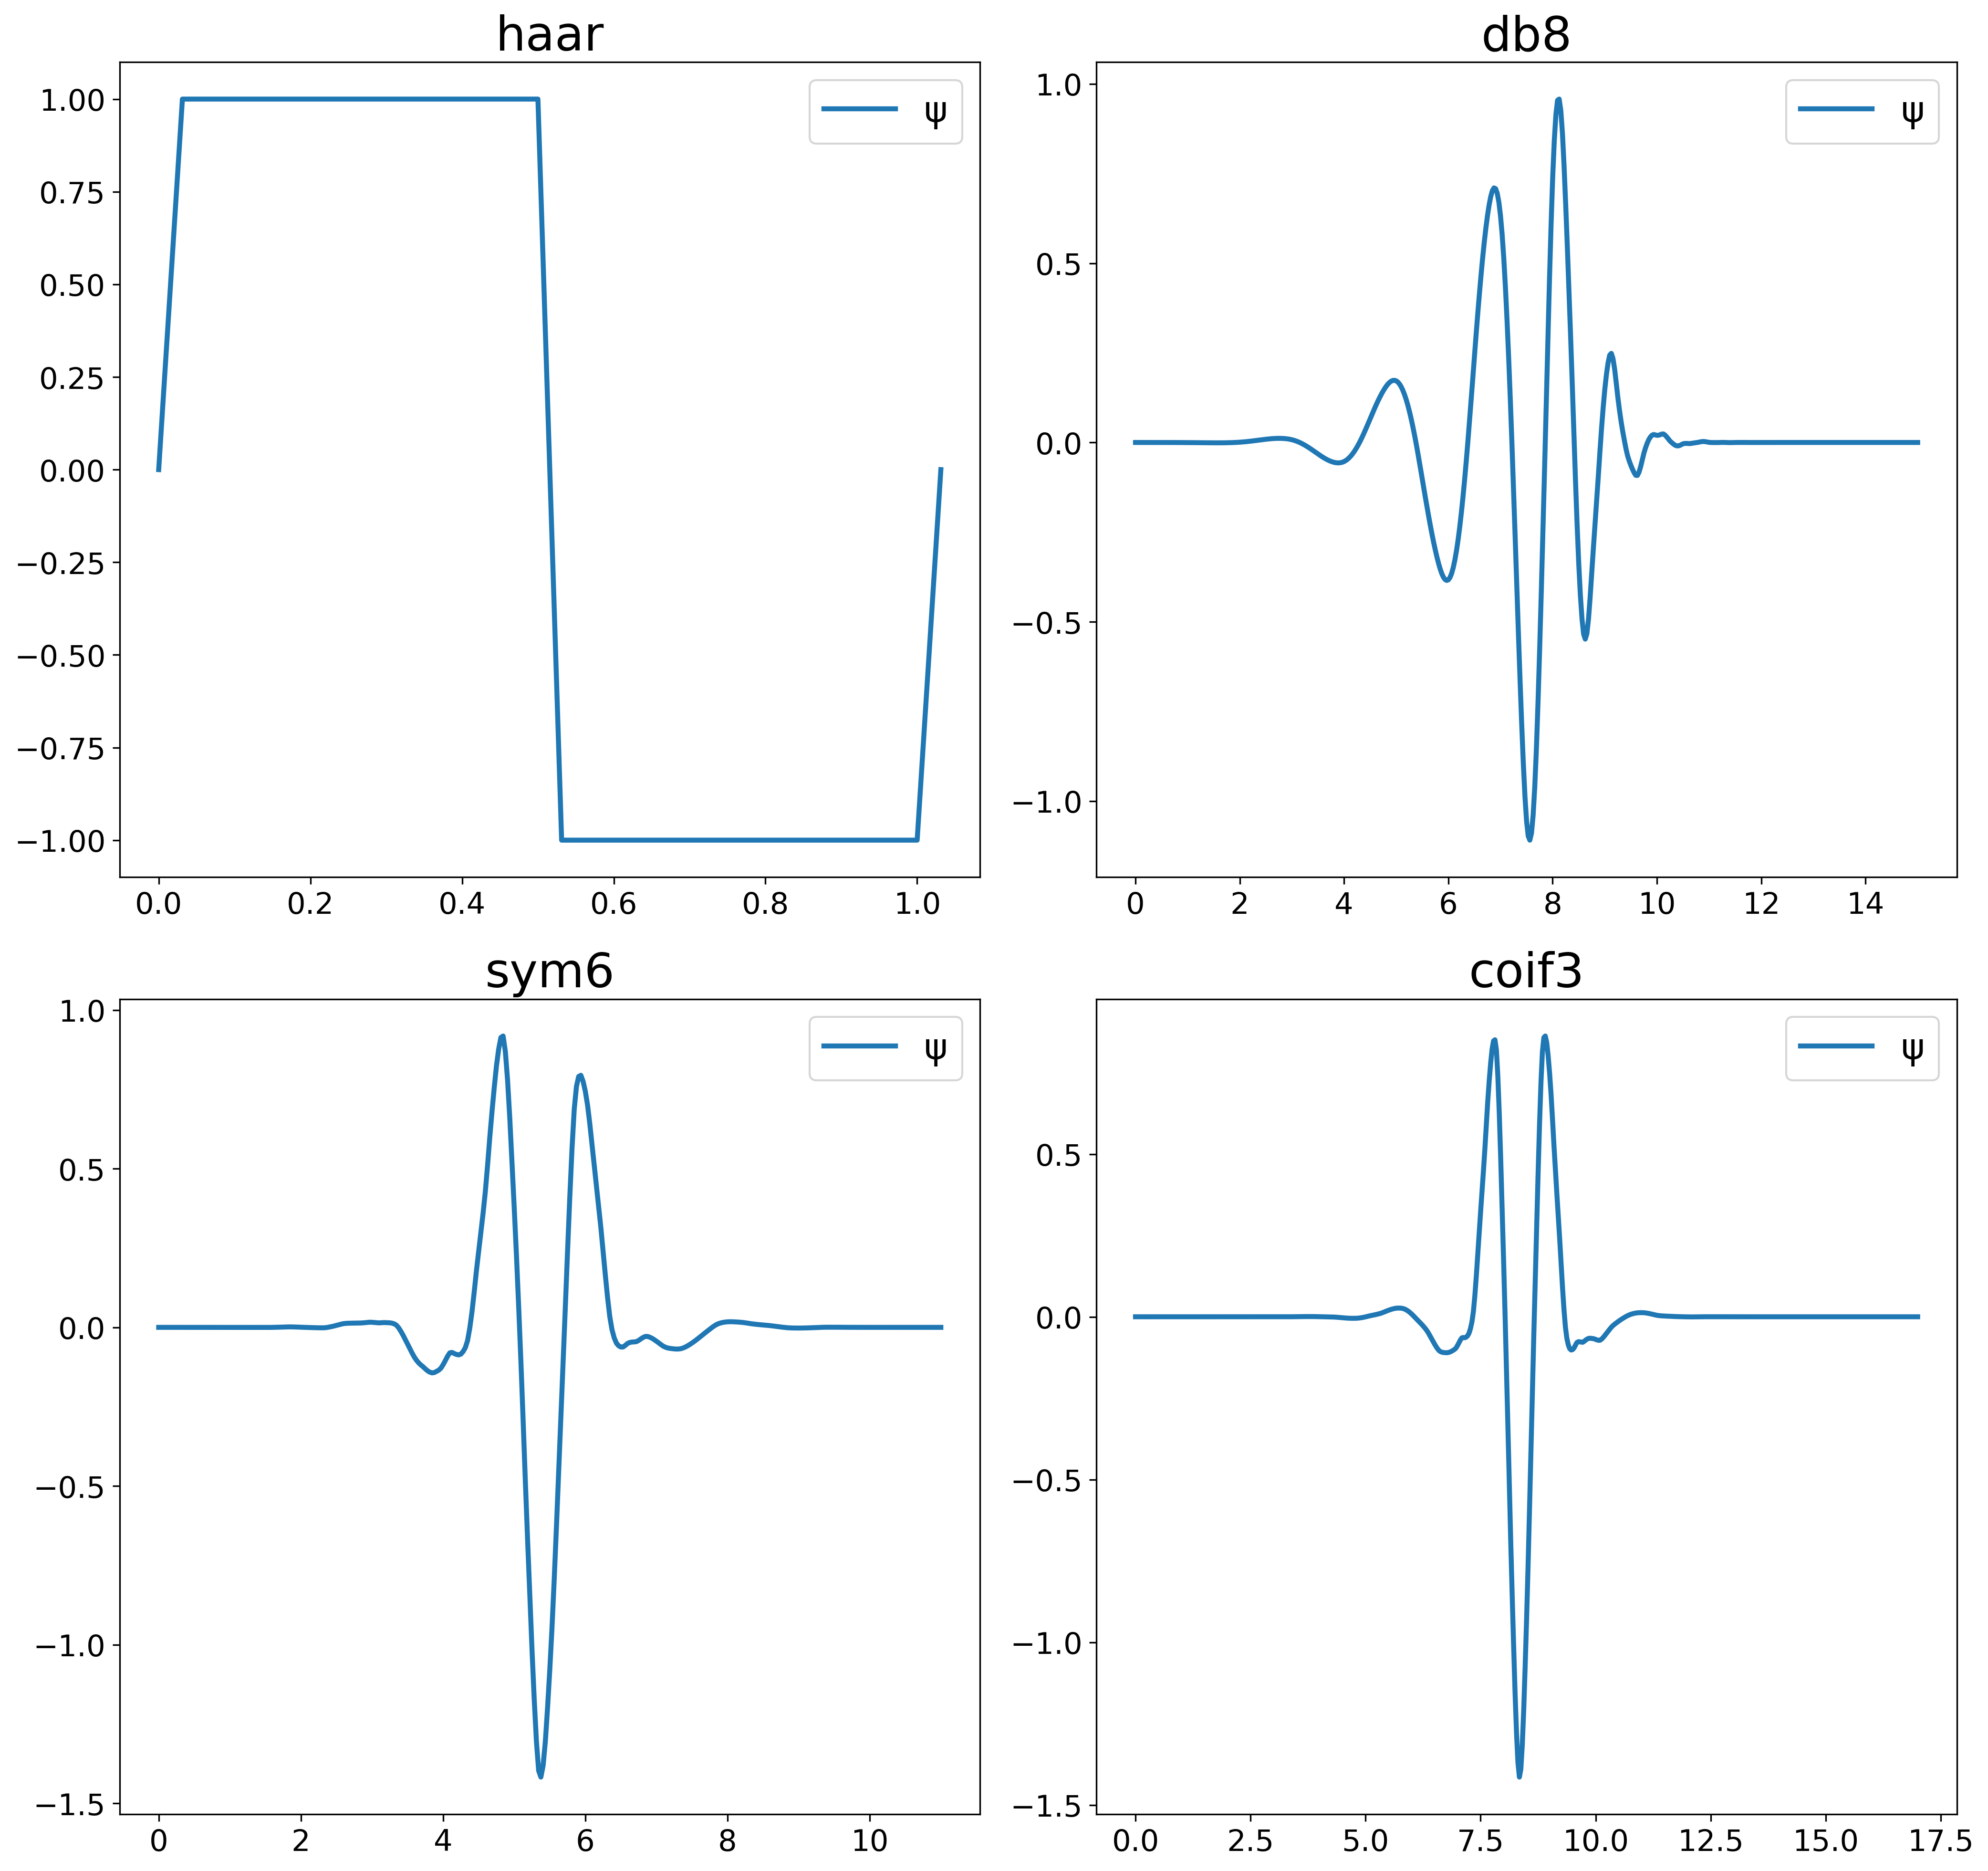
\includegraphics[width=0.60\textwidth]{figures/ch2/wave.png}
\caption{Examples of wavelet generating functions: Haar, Daubechies, Symlets, and Coiflets.}
\label{fig:wavelets}
\end{figure}

Then, the wavelet transform of a signal $f$, denoted by $\check{f}$ at scale $s$ and position $u$, is defined as:
\begin{align}
    \check{f}(u,s) = \int_{-\infty}^{\infty} f(x) \psi_{u,s}(x) dx \quad \Leftrightarrow \quad \check{f}(u,s) = \langle f, \psi_{u,s} \rangle
\end{align}




\subsection{From Continuous to Discrete Wavelets}

The Continuous Wavelet Transform provides a redundant representation of a signal by evaluating wavelet coefficients over a continuous range of translations and scales. While this formulation offers a powerful theoretical framework for time-frequency and multi-scale analysis, it is not directly suitable for numerical applications. Indeed, the parameters $u$ and $s$ can take infinitely many values, leading to an infinite number of wavelet coefficients for a finite signal.

To obtain a finite and computationally tractable representation, the continuous parameter space is discretized. A common choice consists in sampling the scale and translation parameters on a dyadic grid:
\begin{align}
s_j = 2^{-j},
\qquad
u_{j,n} = n 2^{-j},
\end{align}
where $(j,n) \in \mathbb{Z}^2$. The corresponding family of wavelets becomes
\begin{align}
\psi_{j,n}(x)
=
2^{j/2}
\psi\!\left(2^j x - n\right).
\end{align}

The continuous wavelet transform is then replaced by a discrete set of coefficients
\begin{align}
d_{j,n}
=
\langle f,\psi_{j,n}\rangle,
\end{align}
which quantify the contribution of the signal around position $n$ and scale $2^{-j}$. Unlike the continuous transform, this representation contains a finite number of coefficients for a discretized signal and can therefore be manipulated efficiently on a computer.

The dyadic discretization is closely related to the concept of Multi-resolution Analysis (MRA). In this framework, a hierarchy of nested approximation spaces
\begin{align}
\cdots \subset V_{-1}
\subset V_0
\subset V_1
\subset \cdots
\end{align}
is constructed from the scaling function $\phi$. Each space $V_j$ contains approximations of the signal at resolution $2^{-j}$. The information gained when increasing the resolution from $V_j$ to $V_{j+1}$ is represented by a detail space $W_j$, yielding the fundamental decomposition
\begin{align}
V_{j+1}
=
V_j \oplus W_j.
\end{align}

This relation states that a finer approximation can be obtained by adding the detail information contained in $W_j$ to the coarser approximation $V_j$. Consequently, a signal can be decomposed into a coarse approximation together with a collection of detail coefficients at different scales. This hierarchical representation forms the basis of the Discrete Wavelet Transform and enables efficient multi-scale analysis, compression, and denoising algorithms.



\subsection{Fast Discrete Wavelet Transform in Two Dimensions}

The discretization introduced in the previous section leads to an efficient algorithm for computing wavelet coefficients known as the Fast Wavelet Transform (FWT). Rather than explicitly evaluating inner products with every wavelet basis function, the transform relies on successive filtering operations derived from the Multi-resolution Analysis framework.

For a one-dimensional signal, two complementary filters are applied at each decomposition level:

\begin{itemize}
    \item a low-pass filter associated with the scaling function $\phi$, producing approximation coefficients,
    \item a high-pass filter associated with the wavelet function $\psi$, producing detail coefficients.
\end{itemize}

After filtering, the outputs are downsampled by a factor of two. Denoting by $a_j[n]$ the approximation coefficients at level $j$, the decomposition can be written as

\begin{align}
a_{j+1}[n]
&=
\sum_k h[k] a_j[2n-k], \\
d_{j+1}[n]
&=
\sum_k g[k] a_j[2n-k],
\end{align}

where $h[k]$ and $g[k]$ represent the low-pass and high-pass filter coefficients, respectively. The approximation coefficients capture the large-scale structure of the signal, while the detail coefficients describe localized variations at the corresponding scale. 

Figure \ref{fig:wavelet_1d_example} illustrates the decomposition of a one-dimensional signal using a discrete wavelet transform with Haar wavelets. The original signal is decomposed into approximation and detail coefficients, revealing the hierarchical structure of the data across multiple scales.


\begin{figure}[H]
\centering
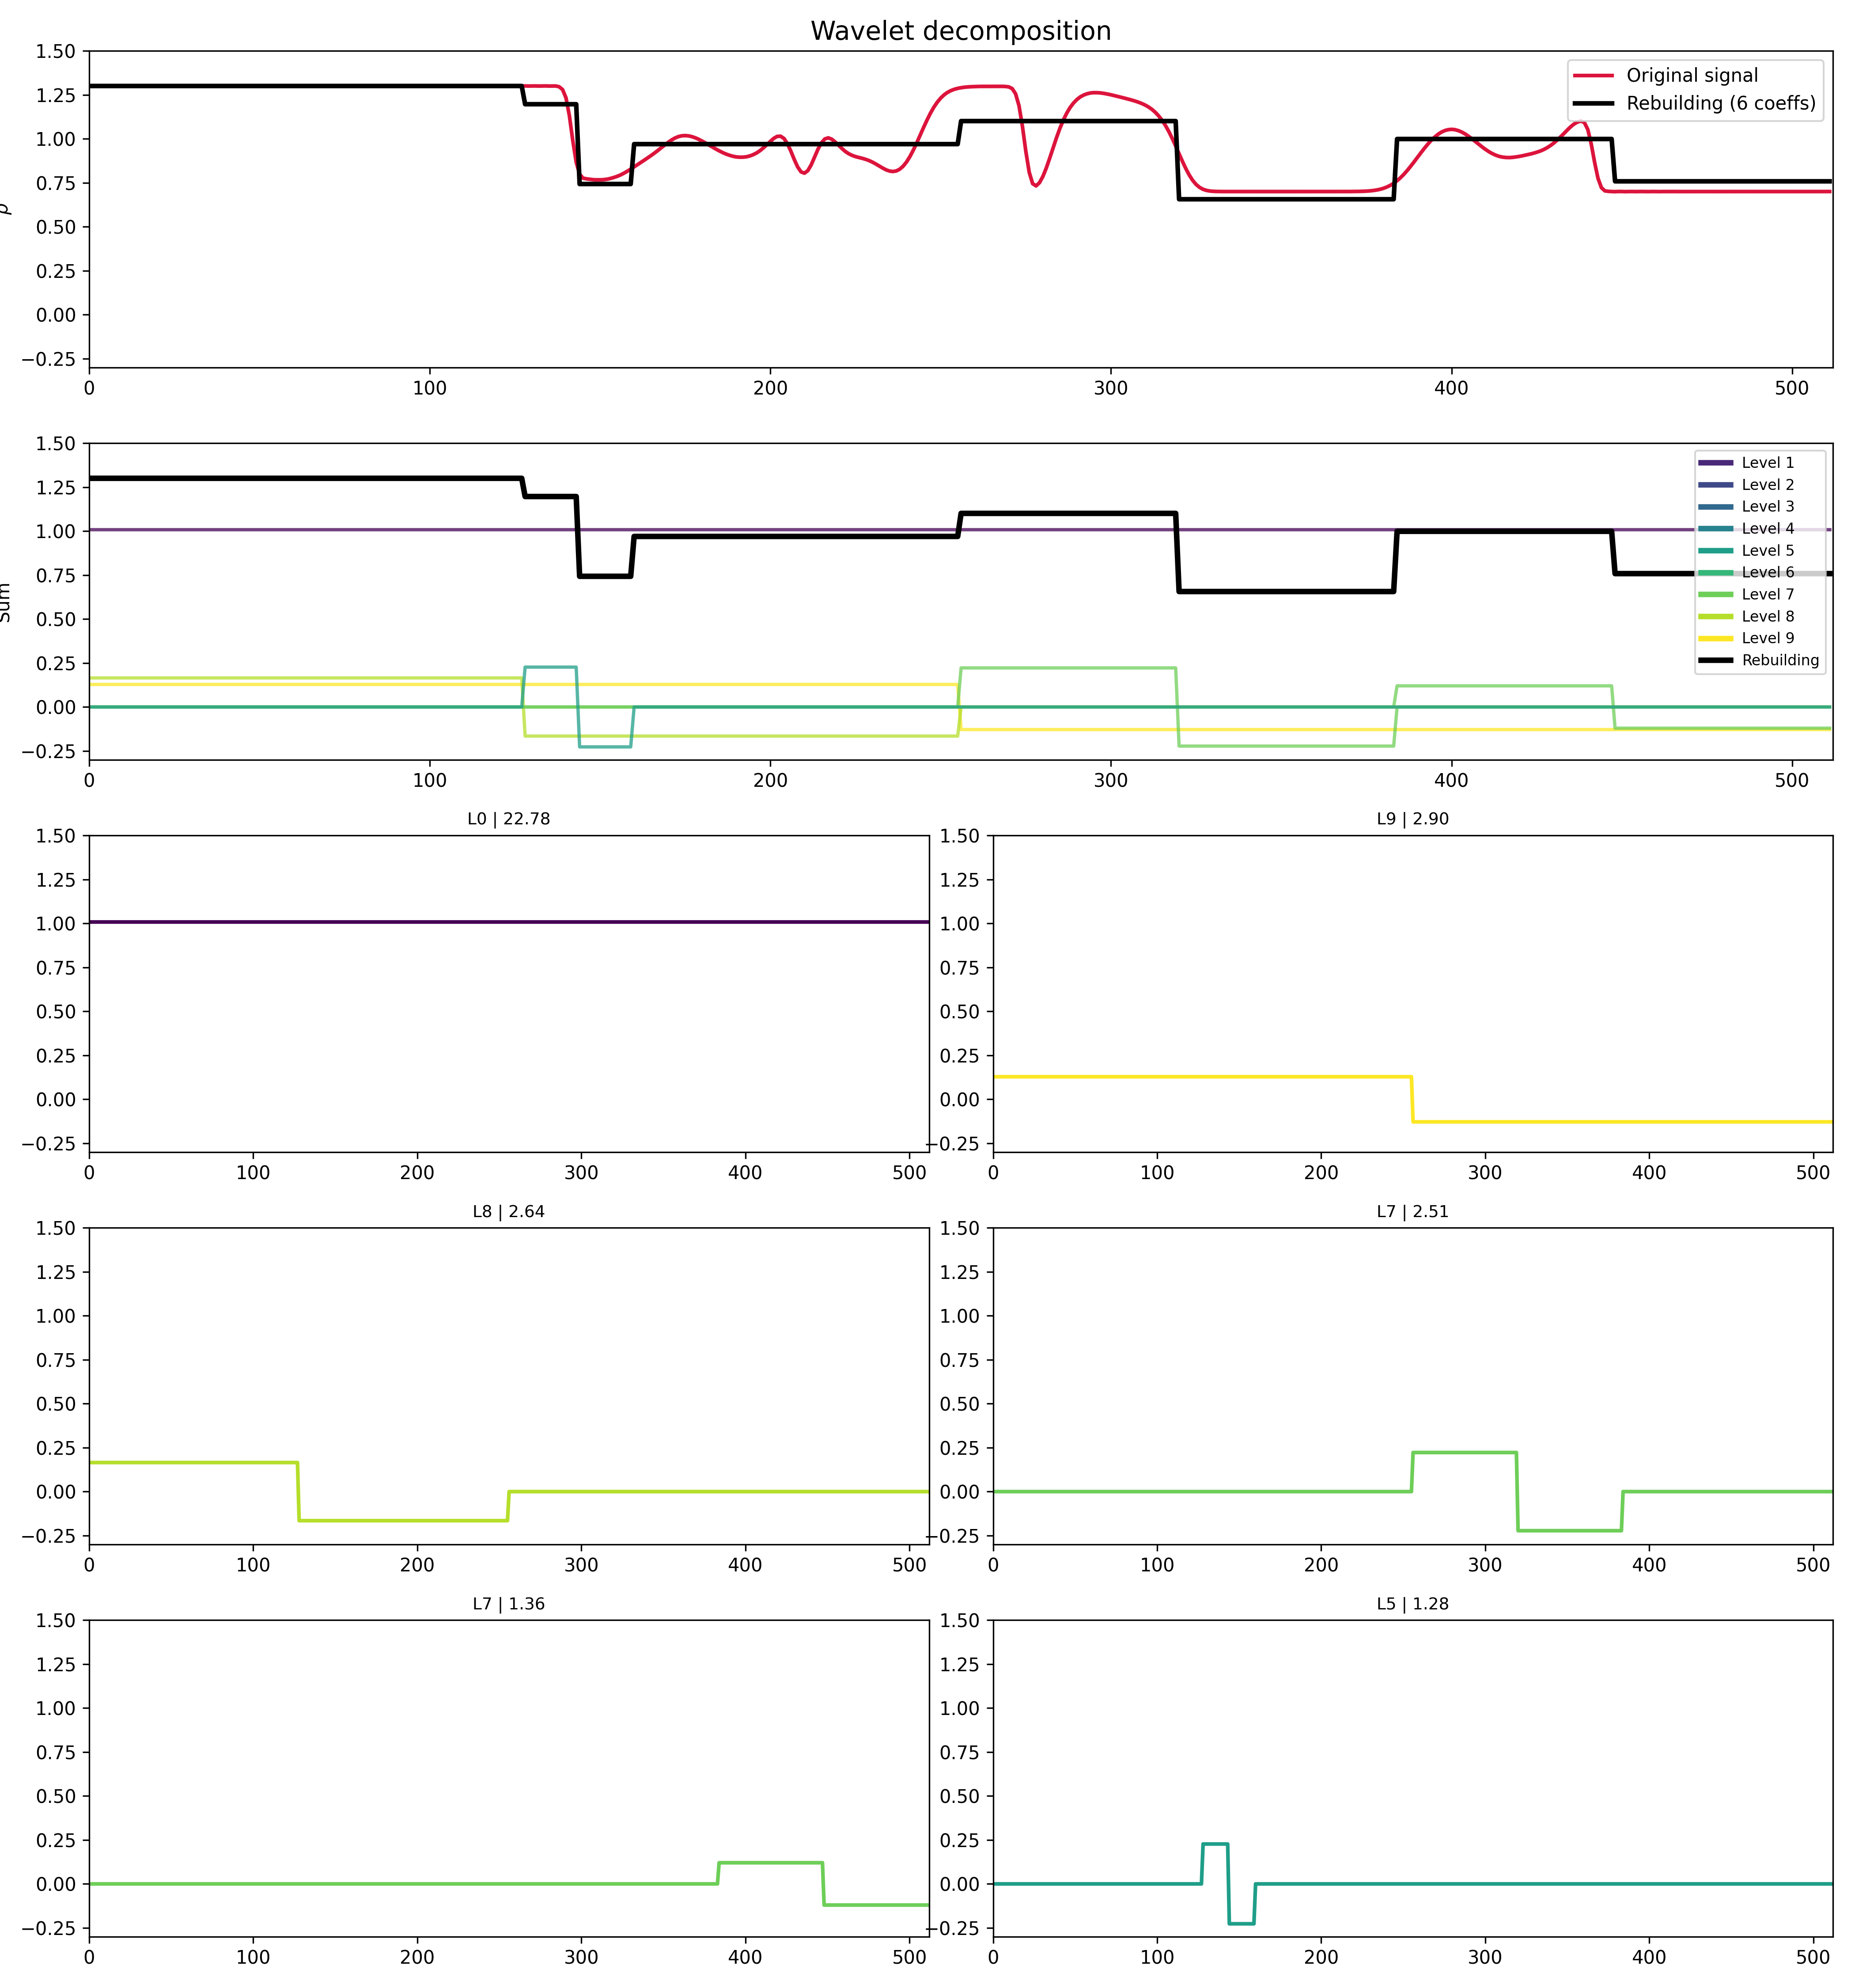
\includegraphics[width=0.85\textwidth]{figures/ch2/1Dwavelets_Decomposition.png}
\caption{Example of a signal decomposition using a one-dimensional discrete wavelet transform, using Haar wavelets.}
\label{fig:wavelet_1d_example}
\end{figure}

For two-dimensional fields, the same principle is applied successively along the horizontal and vertical directions. The image is first filtered row-wise and downsampled, then the resulting intermediate fields are filtered column-wise. This separable construction yields four groups of coefficients:

\begin{align}
LL,\quad LH,\quad HL,\quad HH.
\end{align}

The $LL$ component corresponds to low-pass filtering in both directions and therefore contains a coarse approximation of the original field. The three remaining components contain directional details:

\begin{itemize}
\item $LH$: low-pass horizontally and high-pass vertically,
\item $HL$: high-pass horizontally and low-pass vertically,
\item $HH$: high-pass filtering in both directions.
\end{itemize}

These sub-bands provide a natural separation of structures according to both scale and orientation. Figure \ref{fig:dwt2d_scheme} summarizes the decomposition process, while Figure \ref{fig:dwt2d_example} presents an example applied to a density field from the RTI dataset.

\begin{figure}[H]
\centering
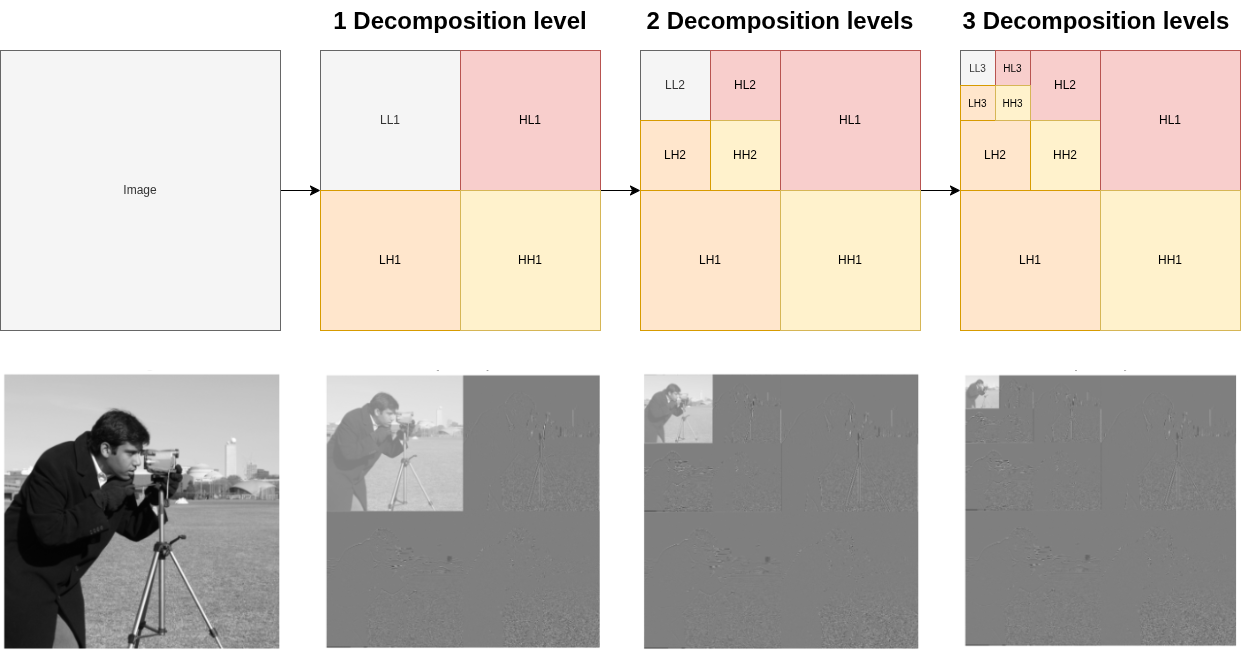
\includegraphics[width=0.8\textwidth]{figures/ch2/wavelet_decomposition.png}
\caption{Schematic representation of a two-dimensional discrete wavelet decomposition.}
\label{fig:dwt2d_scheme}
\end{figure}

\begin{figure}[H]
\centering

\includegraphics[width=0.65\textwidth]{figures/ch2/2DExemple_Masque.png}
\caption{Example of a one-level two-dimensional wavelet decomposition of an RTI density field. The approximation coefficients ($LL$) contain the large-scale structures, while the $LH$, $HL$, and $HH$ sub-bands capture progressively finer directional information.}
\label{fig:dwt2d_example}
\end{figure}

% An important property of this decomposition is that most of the signal energy is generally concentrated within the approximation coefficients, whereas many detail coefficients exhibit relatively small amplitudes. This sparsity property is one of the main reasons why wavelet representations are widely used for compression and multi-scale modeling. In the present work, the $LL$ coefficients are interpreted as a low-resolution representation of the density field and are used as conditioning information for a diffusion model trained to reconstruct the missing detail coefficients. The complete field can then be recovered through the inverse wavelet transform.

\subsection{Compression and Sparsity}

One important property of wavelet representations is their ability to produce sparse decompositions for signals containing localized structures or coherent patterns. A large portion of the signal energy can often be concentrated into a relatively small number of significant coefficients.

This property has been extensively exploited in image compression applications such as JPEG2000, where wavelet decompositions provide efficient representations of natural images while preserving localized features.

In the context of RTI simulations, wavelet sparsity may help reduce the effective dimensionality of the dataset while preserving physically important structures such as interfaces, vortices, and localized mixing regions.

Furthermore, the hierarchical organization of wavelet coefficients appears particularly compatible with the multi-scale nature of turbulence and may therefore provide advantageous representations for generative modeling.

\section{Comparaison and Application to RTI Fields}

\subsection{Comparaison Criteria}
In the context of this work, the main criteria for comparing Fourier and wavelet representations are the number of coefficients required to accurately reconstruct the signal, the ability to capture localized structures and sharp gradients, the effectiveness of separating structures across different scales, and the generalization capabilities to unseen data or different flow regimes. Figure \ref{fig:representation_comparison} illustrates the reconstruction of a two-dimensional Rayleigh--Taylor density field using Fourier, wavelet, and PCA representations with the same number of coefficients. The comparison highlights the differences in capturing sharp gradients and gibbs-like oscillations.
It is also important to note that the PCA is used here as a reference for comparison, but it is not a practical solution for generative modeling since it requires access to the entire training dataset and does not provide extrapolation capabilities for unseen samples.

\begin{figure}[h]
\centering
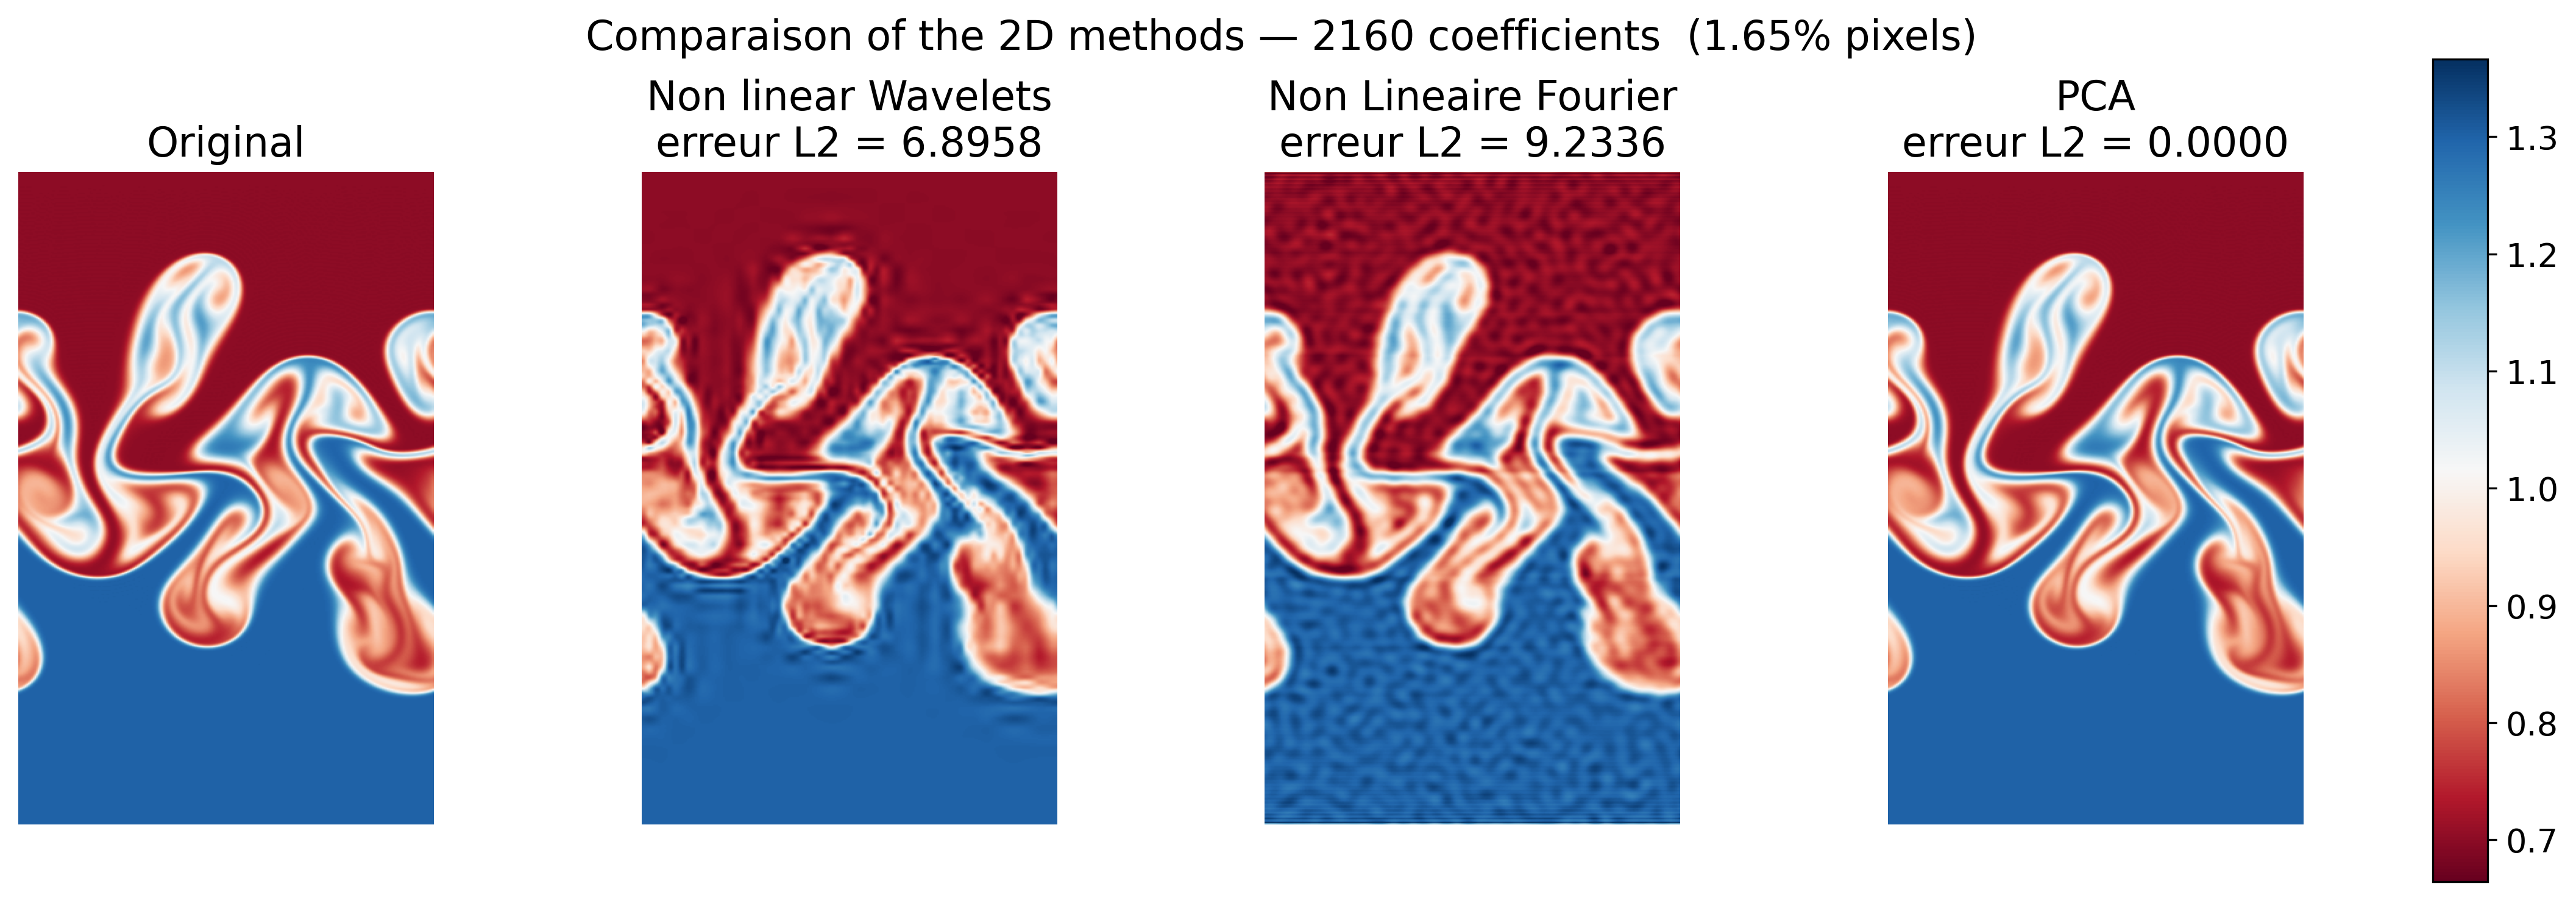
\includegraphics[width=0.9\textwidth]{figures/ch2/verification_zone_melange.png}
\caption{Comparison of different representations for a two-dimensional Rayleigh--Taylor density field}
\label{fig:representation_comparison}
\end{figure}

For more quantitative comparisons, the reconstruction error is computed as the L2 norm between the original field and its reconstruction. Figure \ref{fig:representation_error_comparison} shows the evolution of the reconstruction error as a function of the number of coefficients for Fourier, wavelet, and PCA representations. The results indicate that wavelet representations generally provide better reconstruction after a certain number of coefficients having a very steep decrease of the error.

\begin{figure}[h]
\centering
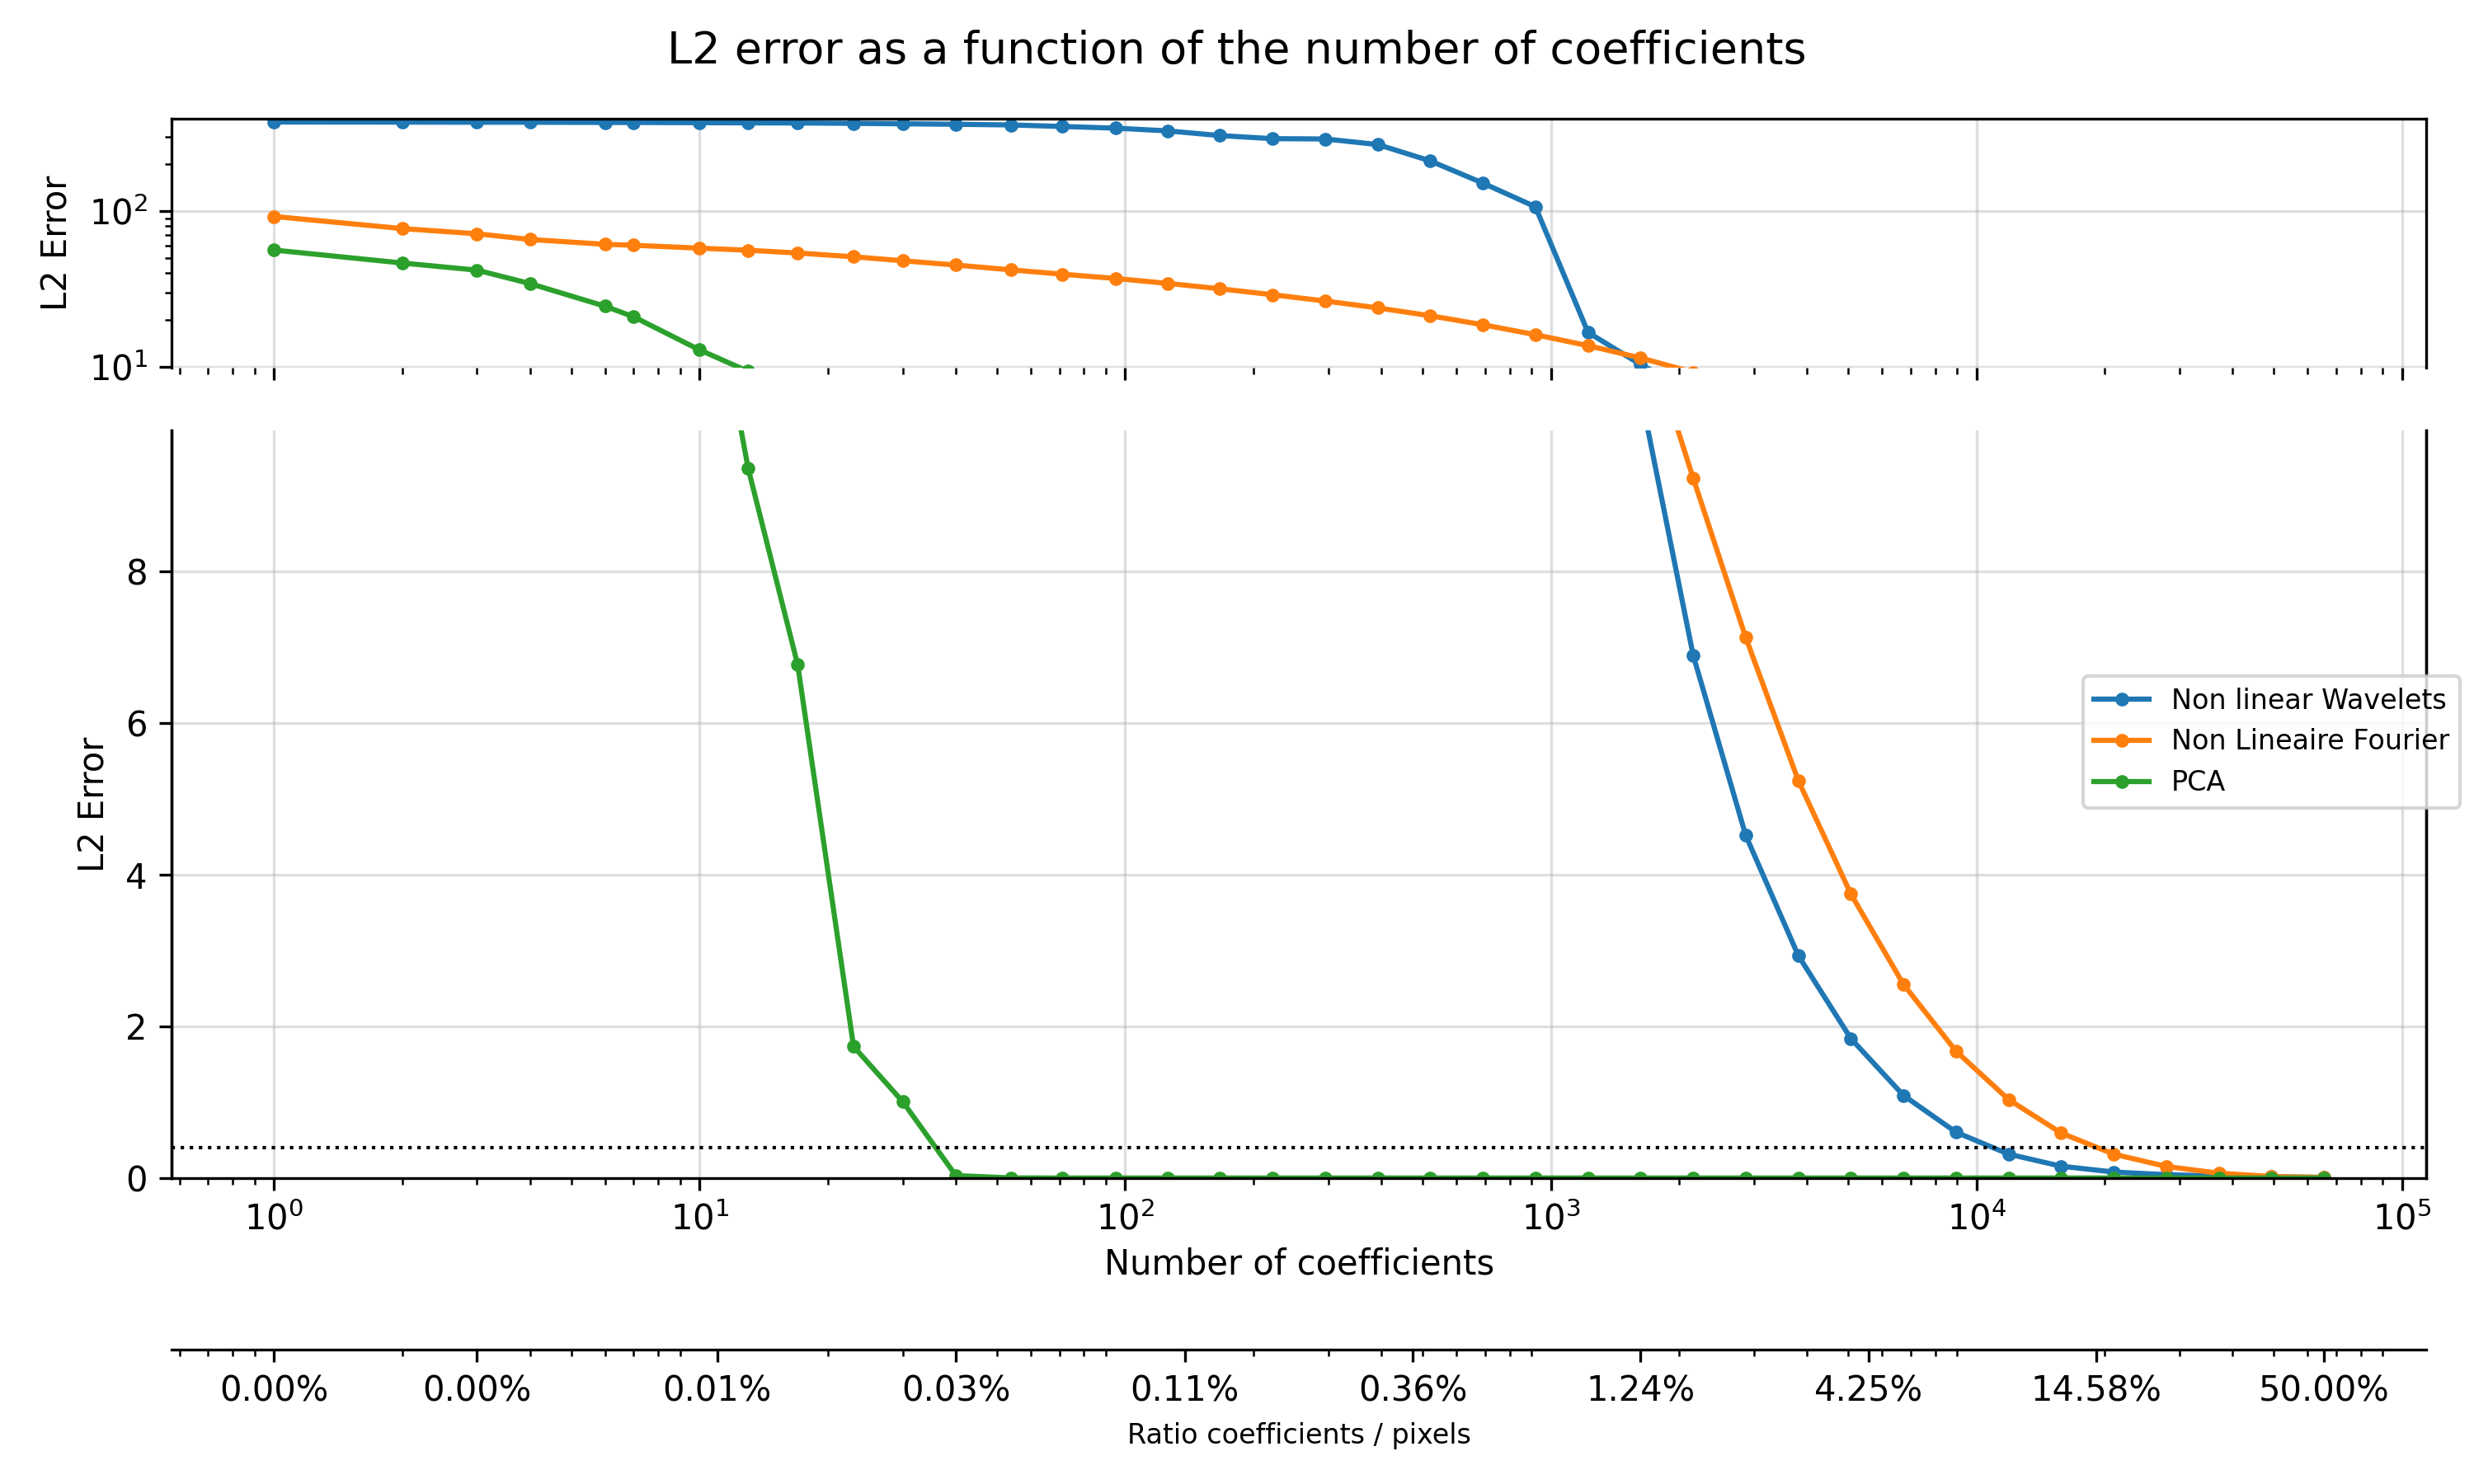
\includegraphics[width=0.65\textwidth]{figures/ch2/dataset2D_Comparaison_des_Erreurs.png}
\caption{Comparison of different representations for a two-dimensional Rayleigh--Taylor density field}
\label{fig:representation_error_comparison}
\end{figure}

With the same number of coefficients, wavelet representations generally provide better reconstruction of localized structures and sharp gradients compared to Fourier representations. It is for sure less performing than PCA, but it is more robust and independent of the training dataset. The multi-scale nature of wavelet decompositions also allows for a more natural separation of structures across different scales, which is particularly relevant for turbulent RTI flows.

\section{Diffusion Models for RTI Fields}

\section{Introduction to score-based diffusion}

\subsection{From individual simulations to a probability distribution}

Machine learning approaches can broadly be divided into supervised and unsupervised methods. In supervised learning, the objective is to learn a mapping between an input and a target output provided through labeled examples. Typical applications include regression and classification tasks, where each sample is associated with a known quantity of interest.

The objective of the present work is fundamentally different. Given a collection of Direct Numerical Simulations (DNS) of Rayleigh--Taylor instability (RTI), no unique target field is associated with a given realization. Instead, the goal is to learn the statistical structure of the dataset itself and to generate new physically plausible density fields. This places the problem within the framework of unsupervised generative modeling, where the objective is to approximate the probability distribution from which the observed simulations are drawn.

Let $\mathbf{x}_0\in\mathbb{R}^{d}$ denote a discretized RTI density field, or equivalently a vector containing the coefficients of one of the reduced representations introduced in Chapter~2.

\begin{equation}
    \mathcal{D}=\left\{\mathbf{x}_0^{(i)}\right\}_{i=1}^{N}
\end{equation}

is regarded as a finite collection of samples drawn from an unknown data
distribution $p_{\mathrm{data}}(\mathbf{x}_0)$. The central objective is therefore not to reconstruct one particular DNS realization, but to
learn the \emph{the probability distribution} of the simulated RTI
fields. In other words, the model should map the space of admissible density fields to a probability measure that captures the properties of the dataset.
The learned model, denoted by $p_{\theta}(\mathbf{x}_0)$, should approximate the
unknown distribution according to

\begin{equation}
    p_{\theta}(\mathbf{x}_0)\approx
    p_{\mathrm{data}}(\mathbf{x}_0).
\end{equation}

Once trained, it must be possible to draw new samples
$\widetilde{\mathbf{x}}_0\sim p_{\theta}$ that are not copies of the training
fields, while preserving their relevant statistical and physical properties.
For RTI, these properties include the morphology of bubbles and spikes, the
location and thickness of the mixing layer, the distribution of density values,
and the organization of structures across spatial scales. Thus, the quality of
the surrogate cannot be assessed from the visual fidelity of a single generated
field alone; it must also be evaluated by statistical comparison of reference density fields and generated samples.

Directly estimating $p_{\mathrm{data}}$ is challenging because it belongs
to a high-dimensional space and the available number of DNS realizations is limited.
Diffusion model current this difficulty by defining a foward process that gradually transforms the complex dataset into a simple Gaussian distribution. The model then learns to reverse this process, to recover samples from the original distribution.

%%%%%%%%%%%%%%%%%%%%%%%%%%%%%%%%%%%%%%%%%%%%%%%%%%%%%%%%%%%%%%

\subsection{One-dimensional illustrative example}

Before considering RTI fields, it is useful to look at the same mechanism in
one dimension, where the whole probability distribution can be plotted. Let's use a toy dataset sampled from a
mixture of two Gaussian distributions,

\begin{equation}
    p_{\mathrm{data}}(x_0)
    =
    \sum_{k=1}^{2}
    \pi_k\,
    \mathcal{N}(\mu_k,\sigma_k^2),
\end{equation}

with modes centered around $\mu_1=-4$ and $\mu_2=4$. This distribution is
simple enough to visualize, but it already contains the main difficulty faced
by a generative model: the data are not concentrated around a single average
state. The model must instead represent two separated regions of high
probability, as illustrated in Figure~\ref{fig:diffusion_1d_dataset}.

\begin{figure}[H]
    \centering
    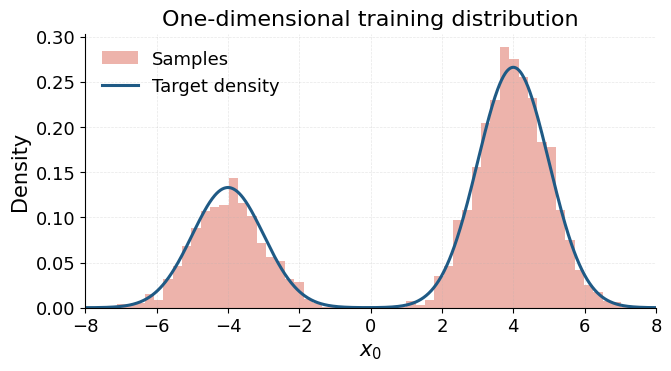
\includegraphics[width=0.70\textwidth]{figures/ch3/diffusion_1d_dataset.png}
    \caption{One-dimensional toy distribution used to illustrate diffusion.
    The histogram represents samples drawn from a bimodal Gaussian mixture,
    while the curve shows the corresponding probability density.}
    \label{fig:diffusion_1d_dataset}
\end{figure}

%%%%%%%%%%%%%%%%%%%%%%%%%%%%%%%%%%%%%%%%%%%%%%%%%%%%%%%%%%%%%%

\subsection{Forward diffusion process}

Following the unified framework introduced by \citep{Song2021SDE}, diffusion models can be interpreted as stochastic processes that progressively transform the data distribution into a simple tractable distribution. Let

\begin{equation}
\mathbf{x}_0 \sim p_{\mathrm{data}}
\end{equation}


denote a sample drawn from the unknown distribution of RTI density fields. The forward diffusion process is defined as a continuous-time stochastic differential equation (SDE)

\begin{equation}
d\mathbf{x}
=
\mathbf{f}(\mathbf{x},t)dt
+
g(t)d\mathbf{w}
\end{equation}

where $(t\in[0,T])$, $(\mathbf{w})$ denotes a standard Wiener process, $(\mathbf{f})$ is a drift coefficient and $(g)$ controls the intensity of the injected noise \citep{Song2021SDE}.

The objective of this process is to progressively destroy the structure present in the data. As time increases, the probability distribution $(p_t(\mathbf{x}))$ evolves from the complex data distribution $(p_{\mathrm{data}})$ toward a simple prior distribution that is chosen as a standard Gaussian,

\begin{equation}
p_T(\mathbf{x})
\approx
\mathcal{N}(\mathbf{0},\mathbf{I}).
\end{equation}

Several choices of forward SDEs are possible. In this work, the implementation is based on the Variance Preserving (VP) formulation, which corresponds to the continuous limit of the Denoising Diffusion Probabilistic Model (DDPM) introduced by \citep{Ho2020DDPM}. In this case, the forward process can be written as

\begin{equation}
d\mathbf{x}
=
-\frac{1}{2}\beta(t)\mathbf{x},dt
+
\sqrt{\beta(t)},d\mathbf{w},
\end{equation}

where $(\beta(t))$ controls the noise schedule.

The discrete implementation used during training relies on a finite number of timesteps $(t\in{0,\ldots,T})$. Defining $\bar{\alpha}_t=\prod_{s=1}^{t}\alpha_s$, the noisy sample at any diffusion time can be obtained directly through

\begin{equation}
\mathbf{x}_t
=
\sqrt{\bar{\alpha}_t},\mathbf{x}_0
+
\sqrt{1-\bar{\alpha}_t},
\boldsymbol{\epsilon},
\qquad
\boldsymbol{\epsilon}
\sim
\mathcal{N}(\mathbf{0},\mathbf{I}).
\end{equation}

This expression reveals the competition between the information contained in the original RTI field and the progressively increasing Gaussian perturbation. For sufficiently large diffusion times, the signal component vanishes and the distribution approaches the Gaussian prior used to initialize the generation process.

This mechanism is illustrated Figure~\ref{fig:diff1d} in
one dimension by a bimodal distribution: its two modes progressively
merge until the samples become approximately Gaussian. The same principle
applies to RTI fields, although their probability distribution lies in a much
higher-dimensional space and cannot be represented by a simple histogram.

\begin{figure}[H]
    \centering
    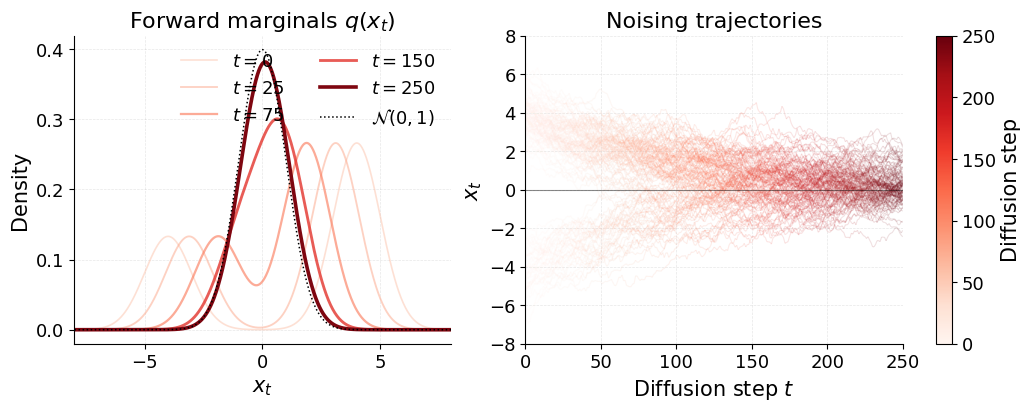
\includegraphics[width=0.95\textwidth]{figures/ch3/diffusion_1d_forward.png}
    \caption{Forward diffusion in one dimension. Left: evolution of the noisy
    marginal density $p_T(\mathbf{x})$ for several diffusion times. Right: trajectories
    of individual samples during the Markov noising process.}
    \label{fig:diff1d}
\end{figure}

%%%%%%%%%%%%%%%%%%%%%%%%%%%%%%%%%%%%%%%%%%%%%%%%%%%%%%%%%%%%%%

\subsection{Learning the Reverse Process Through the Score}

While the forward process is known analytically, the reverse evolution that transforms Gaussian noise back into realistic samples is generally intractable. A central result established by \citep{ANDERSON1982313} and exploited by \citep{Song2021SDE} is that the reverse-time dynamics of the diffusion process is itself governed by a stochastic differential equation,

\begin{equation}
d\mathbf{x}
=
\left[
\mathbf{f}(\mathbf{x},t)
-
g(t)^2
\nabla_{\mathbf{x}}
\log p_t(\mathbf{x})
\right]dt
+
g(t),d\bar{\mathbf{w}},
\end{equation}

where $(d\bar{\mathbf{w}})$ denotes a reverse-time Wiener process and

\begin{equation}
\nabla_{\mathbf{x}}
\log p_t(\mathbf{x})
\end{equation}

is the score function of the perturbed distribution at time (t).

The score corresponds to the gradient of the logarithmic probability density. Geometrically, it points toward regions of higher probability and therefore indicates how a noisy sample should be displaced in order to become more representative of the underlying data distribution. Consequently, learning the reverse process reduces to estimating the score function at every noise level.

A neural network parameterized by $(\theta)$
\begin{equation}
    p_{\theta}(\mathbf{x}_{0:T})
    =
    p(\mathbf{x}_T)
    \prod_{t=1}^{T}
    p_{\theta}(\mathbf{x}_{t-1}\mid\mathbf{x}_t)
\end{equation}

In the score-based formulation, the network learns the score $\mathbf{s}_{\theta}(\mathbf{x}_t,t)$ of the noisy
distribution,

\begin{equation}
    \mathbf{s}_{\theta}(\mathbf{x}_t,t)
    \approx
    \nabla_{\mathbf{x}_t}\log p_t(\mathbf{x}_t),
\end{equation}

which points toward regions of higher probability density at each noise level.
In practice, an equivalent and commonly used parameterization trains a network
$\boldsymbol{\epsilon}_{\theta}$ to predict the Gaussian noise added to a clean
sample. A simplified training objective is

\begin{equation}
    \mathcal{L}_{\mathrm{simple}}(\theta)
    =
    \mathbb{E}_{\mathbf{x}_0,t,\boldsymbol{\epsilon}}
    \left[
        \left\|
        \boldsymbol{\epsilon}
        -
        \boldsymbol{\epsilon}_{\theta}(\mathbf{x}_t,t)
        \right\|_2^2
    \right].
\end{equation}

Because the model is trained over all noise levels, it learns a sequence of
local denoising directions rather than an explicit analytical expression for
the complex RTI distribution. Repeated application of these directions
transports samples from the Gaussian prior toward the regions occupied by the
DNS data. The resulting ensemble of generated fields provides an approximation
of the distribution sought in this work.

In the one-dimensional setting, figure \ref{fig:diffusion_1d_reverse_score} shows the score can be represented as arrows along
the $x$ axis. These arrows point toward regions where the noisy density is
larger. Near the end of the forward process, the density is almost Gaussian and
the score mainly points back toward the origin. At lower noise levels, the
score separates the samples toward the two modes of the data distribution. The
reverse generative process can therefore be interpreted as a gradual
specialization: an initially structureless Gaussian sample is first brought
back to the high-probability region, then assigned to one of the modes.

\begin{figure}[H]
    \centering
    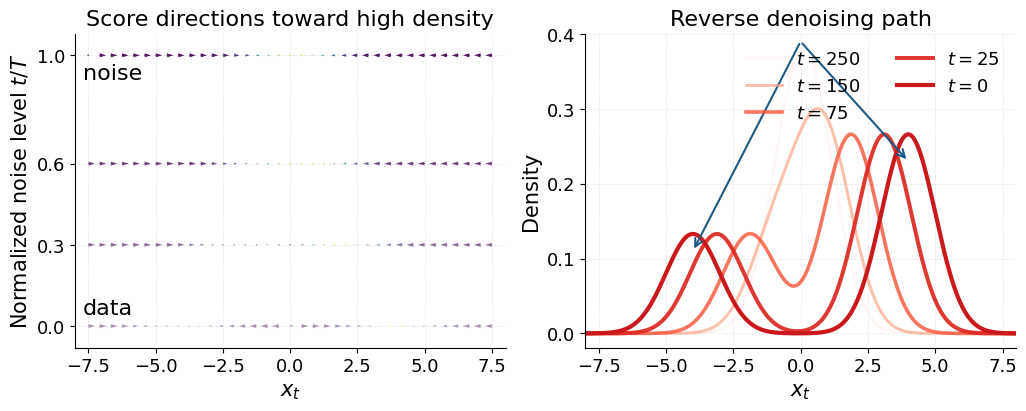
\includegraphics[width=0.95\textwidth]{figures/ch3/diffusion_1d_reverse_score.png}
    \caption{Score-based reverse process in the one-dimensional example. Left:
    score directions for several noise levels. Right: reverse denoising viewed
    as the transformation of the Gaussian prior back into the bimodal data
    distribution.}
    \label{fig:diffusion_1d_reverse_score}
\end{figure}

\begin{equation}
\mathbf{s}*{\theta}(\mathbf{x},t)
\approx
\nabla*{\mathbf{x}}
\log p_t(\mathbf{x}).
\end{equation}

Since the exact score is unknown, it is estimated through denoising score matching. For the variance-preserving formulation adopted in this work, the score can be related to the Gaussian perturbation used during the forward process,
% \citep{Vincent2011,Song2019}


\begin{equation}
\nabla_{\mathbf{x}_t}
\log p(\mathbf{x}_t|\mathbf{x}_0)
=
-
\frac{
\boldsymbol{\epsilon}
}{
\sqrt{1-\bar{\alpha}_t}
}.
\end{equation}

This relation motivates the widely used noise-prediction parameterization introduced by \citet{Ho2020DDPM}, where the neural network predicts the perturbation $(\boldsymbol{\epsilon})$ added to the clean sample. The corresponding training objective is,

\begin{equation}
\mathcal{L}(\theta)
=
\mathbb{E}_{\mathbf{x}*0,t,\boldsymbol{\epsilon}}
\left[
\left|
\boldsymbol{\epsilon}
-
\boldsymbol{\epsilon}*{\theta}
(\mathbf{x}_t,t)
\right|_2^2
\right].
\end{equation}

After training, the estimated score is used to numerically integrate the reverse-time dynamics from an initial Gaussian sample

\begin{equation}
\mathbf{x}_T
\sim
\mathcal{N}(\mathbf{0},\mathbf{I}),
\end{equation}

thereby transporting the probability mass from the simple Gaussian prior toward the complex distribution of RTI density fields. The generated samples can therefore be interpreted as approximate realizations drawn from the learned distribution $(p_{\theta}(\mathbf{x}))$.

%%%%%%%%%%%%%%%%%%%%%%%%%%%%%%%%%%%%%%%%%%%%%%%%%%%%%%%%%%%%%%
%%%%%%%%%%%%%%%%%%%%%%%%%%%%%%%%%%%%%%%%%%%%%%%%%%%%%%%%%%%%%%

\subsection{Conditional diffusion models}

The unconditional formulation above learns a marginal distribution
$p_{\theta}(\mathbf{x}_0)$ and generates samples from Gaussian noise alone.
Many practical settings instead require a \emph{conditional} model, where one
wants to sample from a distribution constrained by external information
$\mathbf{c}$. The objective then becomes

\begin{equation}
    p_{\theta}(\mathbf{x}_0 \mid \mathbf{c}).
\end{equation}

The conditioning variable may be a discrete label, a low-dimensional physical
parameter, or another structured signal. In the simple scalar example used in
the exploratory notebooks, $\mathbf{c}$ is a class label selecting one of two
signal families. In the wavelet setting that will be used in Chapter~4,
$\mathbf{c}$ is instead a coarse approximation coefficient field, while the
variable to be generated is the associated fine-scale detail field.

Figure~\ref{fig:conditional_diffusion_0d_forward} illustrates this idea on a
zero-dimensional toy problem. The marginal dataset is a mixture of several
Gaussian components, but each sample also carries a label $y\in\{0,1\}$. The
forward diffusion process still corrupts the scalar value $x_0$ with Gaussian
noise until the two conditional marginals become almost indistinguishable in
the noisy variable $x_t$. The crucial point is that the label is not diffused:
it remains available to the reverse model as side information.

\begin{figure}[H]
    \centering
    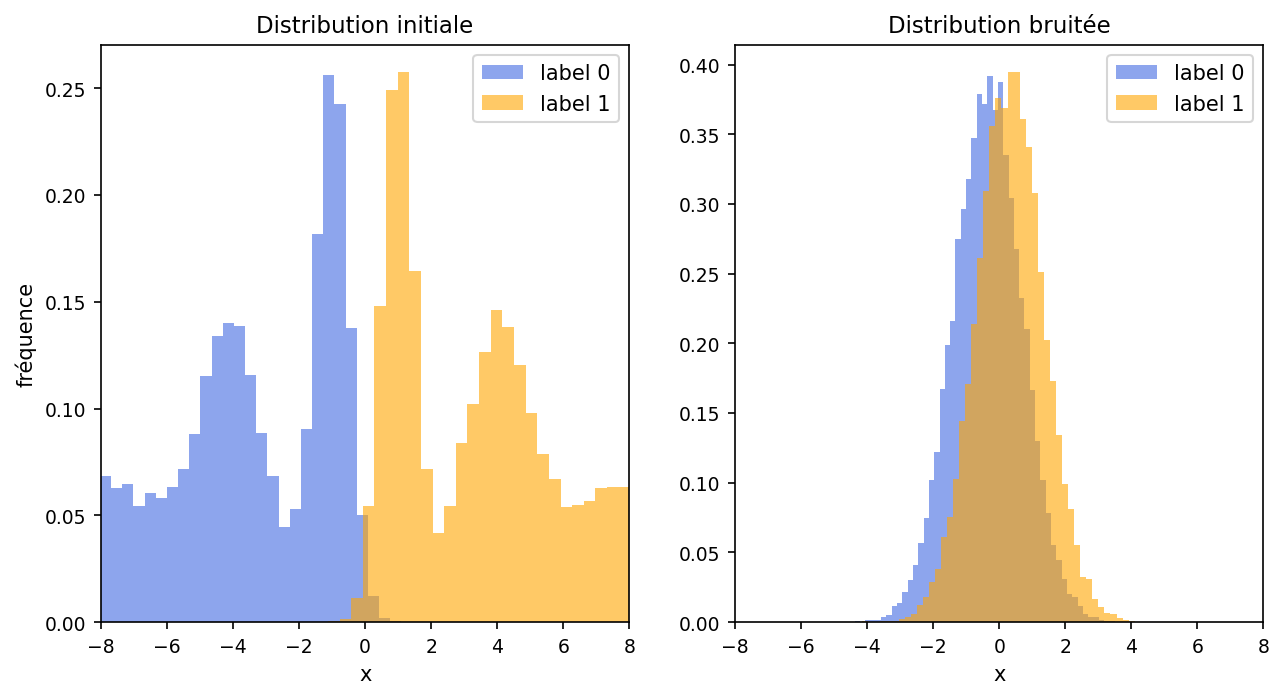
\includegraphics[width=0.85\textwidth]{figures/ch3/conditional_diffusion_0d_forward.png}
    \caption{Forward diffusion in a scalar conditional example. The initial distribution is split into two label-conditioned families. After sufficient noising, the two marginals collapse toward the same Gaussian-like distribution in $x_t$, while the label remains available as conditioning information.}
    \label{fig:conditional_diffusion_0d_forward}
\end{figure}

At the level of the forward process, nothing changes fundamentally: the target
variable is still progressively noised according to the same Markov chain. The
difference appears in the learned reverse model, which now predicts the noise
or the score using both the current noisy sample and the condition,

\begin{equation}
    \boldsymbol{\epsilon}_{\theta}(\mathbf{x}_t,t,\mathbf{c})
    \approx
    \boldsymbol{\epsilon}.
\end{equation}

The corresponding training objective becomes

\begin{equation}
    \mathcal{L}_{\mathrm{cond}}(\theta)
    =
    \mathbb{E}_{\mathbf{x}_0,\mathbf{c},t,\boldsymbol{\epsilon}}
    \left[
        \left\|
        \boldsymbol{\epsilon}
        -
        \boldsymbol{\epsilon}_{\theta}(\mathbf{x}_t,t,\mathbf{c})
        \right\|_2^2
    \right].
\end{equation}

This modification is conceptually simple but important. In an unconditional
model, the network must simultaneously infer the global organization and the
small-scale variability of the data. In a conditional model, part of this
uncertainty is removed by the condition. The model therefore learns a family of
conditional distributions rather than a single global distribution. When the
condition captures the low-frequency organization of the signal, the diffusion
model can focus its capacity on the residual variability compatible with that
coarse structure.

The practical effect is shown in
Figure~\ref{fig:conditional_diffusion_0d_generation}. A conditional network can
generate samples from the two label-conditioned distributions by changing only
the conditioning input. Without this information, an unconditional model would
only learn the marginal mixture and would not provide direct control over which
family is sampled. The conditioning therefore changes the learned reverse
transition from a single denoising field to a collection of denoising fields
indexed by $\mathbf{c}$.

\begin{figure}[H]
    \centering
    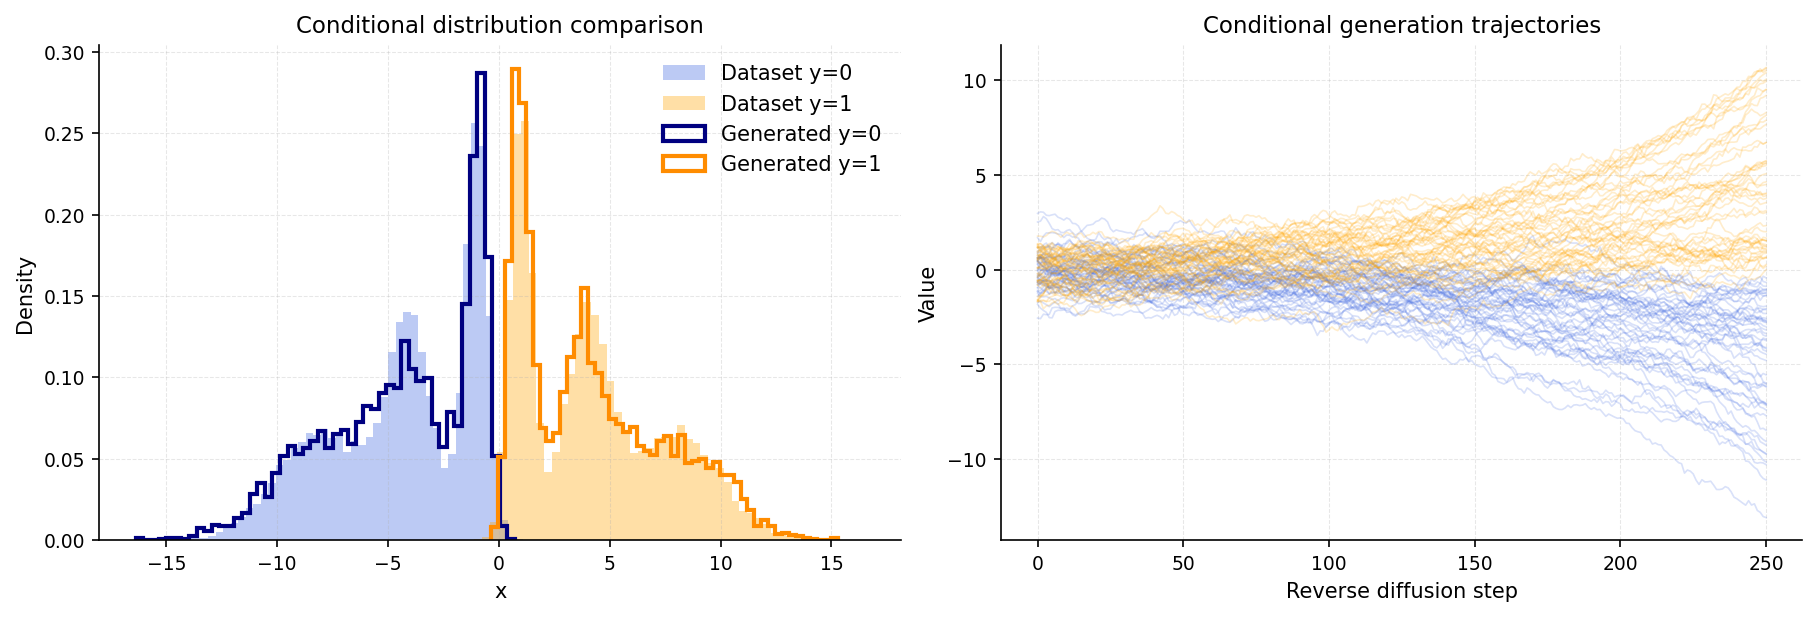
\includegraphics[width=0.95\textwidth]{figures/ch3/conditional_diffusion_0d_generation.png}
    \caption{Conditional generation in the scalar toy example. Left: generated samples reproduce the two target conditional distributions when the label is provided to the model. Right: reverse trajectories starting from Gaussian noise separate according to the prescribed condition.}
    \label{fig:conditional_diffusion_0d_generation}
\end{figure}

This coarse-to-fine factorization is especially relevant for multi-scale
physical fields. For a wavelet decomposition of a signal or image, one may
seek to model

\begin{equation}
    p(\mathbf{x})
    =
    p(\mathbf{c}_A,\mathbf{c}_D)
    =
    p(\mathbf{c}_A)\,p(\mathbf{c}_D\mid\mathbf{c}_A),
\end{equation}

where $\mathbf{c}_A$ denotes approximation coefficients and $\mathbf{c}_D$
detail coefficients. In a deeper cascade, this factorization can be iterated
across scales, for example

\begin{equation}
    p(Ca_3,Ch_3,Ch_2,Ch_1)
    =
    p(Ca_3)\,p(Ch_3\mid Ca_3)\,p(Ch_2\mid Ca_2)\,p(Ch_1\mid Ca_1),
\end{equation}

which is precisely the logic explored in the multi-level wavelet notebooks.
The conceptual gain is that the model no longer needs to generate all scales at
once: coarse content is generated first, then progressively refined by
conditional detail models.

This decomposition does not make the problem trivial. Its usefulness depends on
how informative the condition really is, on whether the chosen architecture can
exploit it effectively, and on whether the coefficient normalization preserves
a reasonable balance between coarse and fine scales. Nevertheless, conditional
diffusion provides the theoretical bridge between the standard DDPM introduced
in this chapter and the wavelet-based methodology described in the next one.

This background chapter introduced the physical, representational, and
algorithmic foundations of the work. The next chapter builds on these elements
to describe the dataset preparation, the implemented training pipelines, and
the conditional wavelet framework used during the internship.
